\documentclass[11pt, letterpaper]{article}

% ── Page Layout ───────────────────────────────────────────────────────────────
\usepackage[margin=1.25in, top=1.2in, bottom=1.2in]{geometry}
\usepackage{setspace}
\setstretch{1.15}
\setlength{\emergencystretch}{6em}
\usepackage{parskip}

% ── Typography ────────────────────────────────────────────────────────────────
\usepackage{iftex}
\ifPDFTeX
  \usepackage[T1]{fontenc}
  \usepackage[utf8]{inputenc}
  \usepackage[scaled=0.95]{helvet}
  \renewcommand{\familydefault}{\sfdefault}
\else
  \usepackage{fontspec}
  \IfFileExists{Poppins-Regular.ttf}{
    \setmainfont{Poppins-Regular.ttf}[
      BoldFont=Poppins-Bold.ttf,
      ItalicFont=Poppins-Italic.ttf,
      BoldItalicFont=Poppins-BoldItalic.ttf
    ]
    \setsansfont{Poppins-Regular.ttf}[
      BoldFont=Poppins-Bold.ttf,
      ItalicFont=Poppins-Italic.ttf,
      BoldItalicFont=Poppins-BoldItalic.ttf
    ]
  }{
    \setmainfont[
      BoldFont=UberMoveBold.otf,
      ItalicFont=UberMoveMedium.otf,
      BoldItalicFont=UberMoveBold.otf
    ]{UberMoveMedium.otf}
    \setsansfont[
      BoldFont=UberMoveBold.otf,
      ItalicFont=UberMoveMedium.otf,
      BoldItalicFont=UberMoveBold.otf
    ]{UberMoveMedium.otf}
  }
  \renewcommand{\familydefault}{\sfdefault}
\fi
\usepackage{microtype}
\usepackage{amsmath, amssymb}
\usepackage{tikz}
\usetikzlibrary{shapes.geometric, calc}

% ── Colours ───────────────────────────────────────────────────────────────────
\usepackage{xcolor}
\definecolor{ink}{HTML}{111827}
\definecolor{muted}{HTML}{4B5563}
\definecolor{blue}{HTML}{1D4ED8}
\definecolor{rule}{HTML}{E5E7EB}
\definecolor{codebg}{HTML}{F3F4F6}
\definecolor{coverbg}{HTML}{C66735}

% ── Section Headings ──────────────────────────────────────────────────────────
\usepackage{titlesec}
\titleformat{\section}
  {\sffamily\Large\bfseries\color{ink}}{}{0em}{}[{\color{rule}\vspace{2pt}\hrule\vspace{4pt}}]
\titlespacing*{\section}{0pt}{3.5ex plus 1ex}{1.5ex}

\titleformat{\subsection}
  {\sffamily\large\bfseries\color{ink}}{}{0em}{}
\titlespacing*{\subsection}{0pt}{2.5ex plus .5ex}{0.6ex}

\titleformat{\subsubsection}
  {\sffamily\normalsize\bfseries\color{muted}}{}{0em}{}
\titlespacing*{\subsubsection}{0pt}{1.8ex}{0.3ex}

% ── Tables & Figures ──────────────────────────────────────────────────────────
\usepackage{booktabs}
\usepackage{caption}
\usepackage{multirow}
\captionsetup{font={sf,small,color=muted}, skip=8pt,
              justification=raggedright, singlelinecheck=false}
\usepackage{graphicx}
\usepackage{float}
\usepackage{subcaption}

% ── Lists ─────────────────────────────────────────────────────────────────────
\usepackage{enumitem}
\setlist[itemize]{itemsep=0.25em, topsep=0.4em, leftmargin=1.4em,
                  label={\color{blue}$\bullet$}}
\setlist[enumerate]{itemsep=0.25em, topsep=0.4em, leftmargin=1.6em}

% ── Links & TOC ───────────────────────────────────────────────────────────────
\usepackage{hyperref}
\hypersetup{colorlinks=true, linkcolor=blue, urlcolor=ink, citecolor=blue}
\usepackage{tocloft}
\renewcommand{\cftsecfont}{\sffamily\bfseries\color{ink}}
\renewcommand{\cftsubsecfont}{\sffamily\color{muted}}
\renewcommand{\cftsecpagefont}{\sffamily\bfseries\color{ink}}
\renewcommand{\cftsubsecpagefont}{\sffamily\color{muted}}
\setlength{\cftbeforesecskip}{6pt}

% ─────────────────────────────────────────────────────────────────────────────
\begin{document}

% ── Cover Page ────────────────────────────────────────────────────────────────
\begin{titlepage}
  \begin{tikzpicture}[remember picture, overlay]

    % Background Fill (Assuming coverbg is defined, otherwise use black!5)
    \fill[coverbg] (current page.south west) rectangle (current page.north east);

    % Title block — upper left
    \node[anchor=north west, inner sep=0pt, xshift=1.2in, yshift=-1.5in]
      at (current page.north west) {
        \begin{minipage}{0.75\paperwidth}
          \raggedright\sffamily\color{black}
          
          % Main Title
          {\fontsize{34}{40}\bfseries\selectfont
            PatchWRAT: Multi-Resolution Transformers\\
            for Time Series Forecasting\par}
          
          \vspace{2.5ex}
          
          % Subtitle
          {\fontsize{16}{22}\selectfont Complete Overview of Proposed Architecture\par}
          
          \vspace{4ex}
          
          % Status and Course Info (Cleaned up, no white box)
          {\fontsize{12}{14}\selectfont\bfseries Final Submission --- May 2026} \\[1.5ex]
          {\fontsize{11}{13}\selectfont\color{black}\uppercase{CS 728 --- Course Work}}
          
        \end{minipage}
      };

    % Metadata block — bottom left
    \node[anchor=south west, inner sep=0pt, xshift=1.2in, yshift=1.5in]
      at (current page.south west) {
        \begin{minipage}{0.75\paperwidth}
          \color{black}
          
          % Bottom Header
          {\fontsize{24}{28}\sffamily\textbf{PatchWRAT}
            \hspace{1.5ex}\vrule width 1.5pt height 18pt depth 2pt\hspace{1.5ex}
            System Overview\par}
          
          \vspace{3ex}
          \hrule height 1pt
          \vspace{4ex}
          
          % Two-column details
          \begin{minipage}[t]{0.56\textwidth}
            \raggedright\sffamily\color{black}
            {\fontsize{9}{11}\selectfont\bfseries\uppercase{Team Members}}\\[1.2ex]
            {\fontsize{13}{17}\bfseries\selectfont Shreyash Wanjari} \hfill {\fontsize{11}{13}\selectfont 22B3926}\\[0.6ex]
            {\fontsize{13}{17}\bfseries\selectfont Pranav Prakash} \hfill {\fontsize{11}{13}\selectfont 22B3945}\\[0.6ex]
            {\fontsize{13}{17}\bfseries\selectfont Akshat Singhvi} \hfill {\fontsize{11}{13}\selectfont 22B1231}\\[3ex]
            
            % {\fontsize{9}{11}\selectfont\bfseries\uppercase{Under the guidance of}}\\[0.8ex]
            % {\fontsize{13}{16}\bfseries\selectfont Prof. Vikram Gadre}\\[3ex]
            
            % {\fontsize{9}{11}\selectfont\bfseries\uppercase{Special thanks}}\\[0.8ex]
            % {\fontsize{11}{13}\selectfont Animesh Kumar, Abhijat Bharadwaj, Inderjeet Sir}
          \end{minipage}
          \hfill
        %   \begin{minipage}[t]{0.42\textwidth}
        %     \raggedleft\sffamily\color{black}
        %     {\fontsize{11}{15}\selectfont
        %       \textbf{Department of Electrical Engineering}\\[0.5ex]
        %       Indian Institute of Technology, Bombay\\[0.5ex]
        %       2026\par}
        %   \end{minipage}
        \end{minipage}
      };

  \end{tikzpicture}
\end{titlepage}

\clearpage
\tableofcontents
\clearpage

% ─────────────────────────────────────────────────────────────────────────────
\section{Problem Description}

\subsection{Motivation}

Forecasting multivariate time series sits at the core of high-stakes decisions across energy grids, climate systems, healthcare, and finance. When a model can reliably say ``load will spike in six hours,'' a grid operator can act; when it cannot, the cost is measured in blackouts or wasted resources. Google's flood-forecasting system in India has already sent over 100 million early warnings reaching an estimated 360 million people, and studies suggest it can cut flood-related damages by 30--50\%. Better forecasting saves real lives.

\subsection{What Is Broken in Current Approaches}

The community currently sits between two unsatisfying extremes. Classical statistical models (ARIMA, SARIMA, VAR) are transparent and interpretable but collapse on long horizons and non-linear patterns. Large Transformer-based models (Informer, Autoformer, FEDformer, iTransformer) achieve impressive accuracy but behave as black boxes --- when wrong, nobody can say why. Both families also struggle with \emph{distribution shift}: real-world signals change their statistical character over time, so a model calibrated on last year's data may silently fail on this year's.

\subsection{The Core Research Question}

Can a compact, \emph{interpretable} model match the accuracy of much larger Transformers by exploiting the known multi-resolution structure of time series? Specifically, can we teach a network to \emph{learn} the frequency separation that classical signal processing imposes by hand, and then route each frequency band to the attention mechanism best suited for it?

\subsection{Proposed Solution: PatchWRAT}

PatchWRAT (\textbf{Patch Wavelet Routing Attention Transformer}) answers this question. Its central argument is that a time series is a mixture of slow, smooth trends and fast, spiky events. Classical signal processing has known how to separate these regimes for decades through the Discrete Wavelet Transform (DWT). PatchWRAT parameterises this decomposition as learnable convolutional filters and handles each frequency band with a dedicated attention mechanism, yielding a model that is both accurate and mathematically transparent.

% ─────────────────────────────────────────────────────────────────────────────
\section{Dataset Used}

\subsection{ETTm1 --- Electricity Transformer Temperature (15-min)}

All experiments use the \textbf{ETTm1} benchmark, a widely adopted standard in the long-horizon forecasting literature.

\begin{itemize}
  \item \textbf{Source:} Publicly available ETT (Electricity Transformer Temperature) dataset, originally published alongside the Informer paper (Zhou et al., 2021).
  \item \textbf{Variates ($C=7$):} High/mid/low useful load (HUFL, MUFL, LUFL), high/mid/low load (HULL, MULL, LULL), and oil temperature (OT).
  \item \textbf{Sampling Rate:} Every 15 minutes.
  \item \textbf{Total Length:} Approximately 69,680 timesteps spanning roughly two years.
  \item \textbf{Input Sequence Length:} $L = 512$ timesteps ($\approx$5.3 days of context).
  \item \textbf{Prediction Horizons:} $H \in \{96, 192, 336, 720\}$ steps (1 day to 7.5 days ahead).
\end{itemize}

\subsection{Preprocessing Pipeline}

Two normalisation stages are applied in sequence:

\begin{enumerate}
  \item \textbf{Global StandardScaler:} A \texttt{sklearn.preprocessing.StandardScaler} is fit on the training split and applied to train, validation, and test splits. This removes the mean and scales to unit variance across the full dataset.
  \item \textbf{Per-sample RevIN:} At inference time, each input window is independently normalised (zero mean, unit variance) and the prediction is inverted back to physical scale. This second stage handles local distributional shifts that the global scaler cannot.
\end{enumerate}

\textbf{Data splits} follow the chronological 60/20/20 convention: 60\% train, 20\% validation, 20\% test. No shuffling is applied; temporal order is strictly preserved.

% ─────────────────────────────────────────────────────────────────────────────
\section{Architecture and Implementation}

\subsection{Three Core Contributions}

\begin{enumerate}
  \item \textbf{Learnable 1D Discrete Wavelet Transform.} Rather than hard-coding a Haar or Daubechies basis, PatchWRAT parameterises the low-pass and high-pass filter banks as 1D convolutional layers (stride 2) and lets the network discover the wavelet shape that best fits the dataset.

  \item \textbf{Dual-path attention routing via the WRATBlock.} The decomposed low-frequency ($LL$) and high-frequency ($LH$) subbands are routed through different attention mechanisms. Dense self-attention captures global structure in $LL$; dynamically thresholded sparse attention in $LH$ acts as a noise gate, attending only to statistically significant events. A cross-attention layer then fuses the two representations.

  \item \textbf{Orthogonality loss for structural regularisation.} A penalty on the dot product between the learned filters ensures they remain mathematically independent, preserving the wavelet property that $LL$ and $LH$ together reconstruct the original signal without information loss.
\end{enumerate}

\subsection{Forward Pass: Four Stages}

\begin{figure}[H]
  \centering
  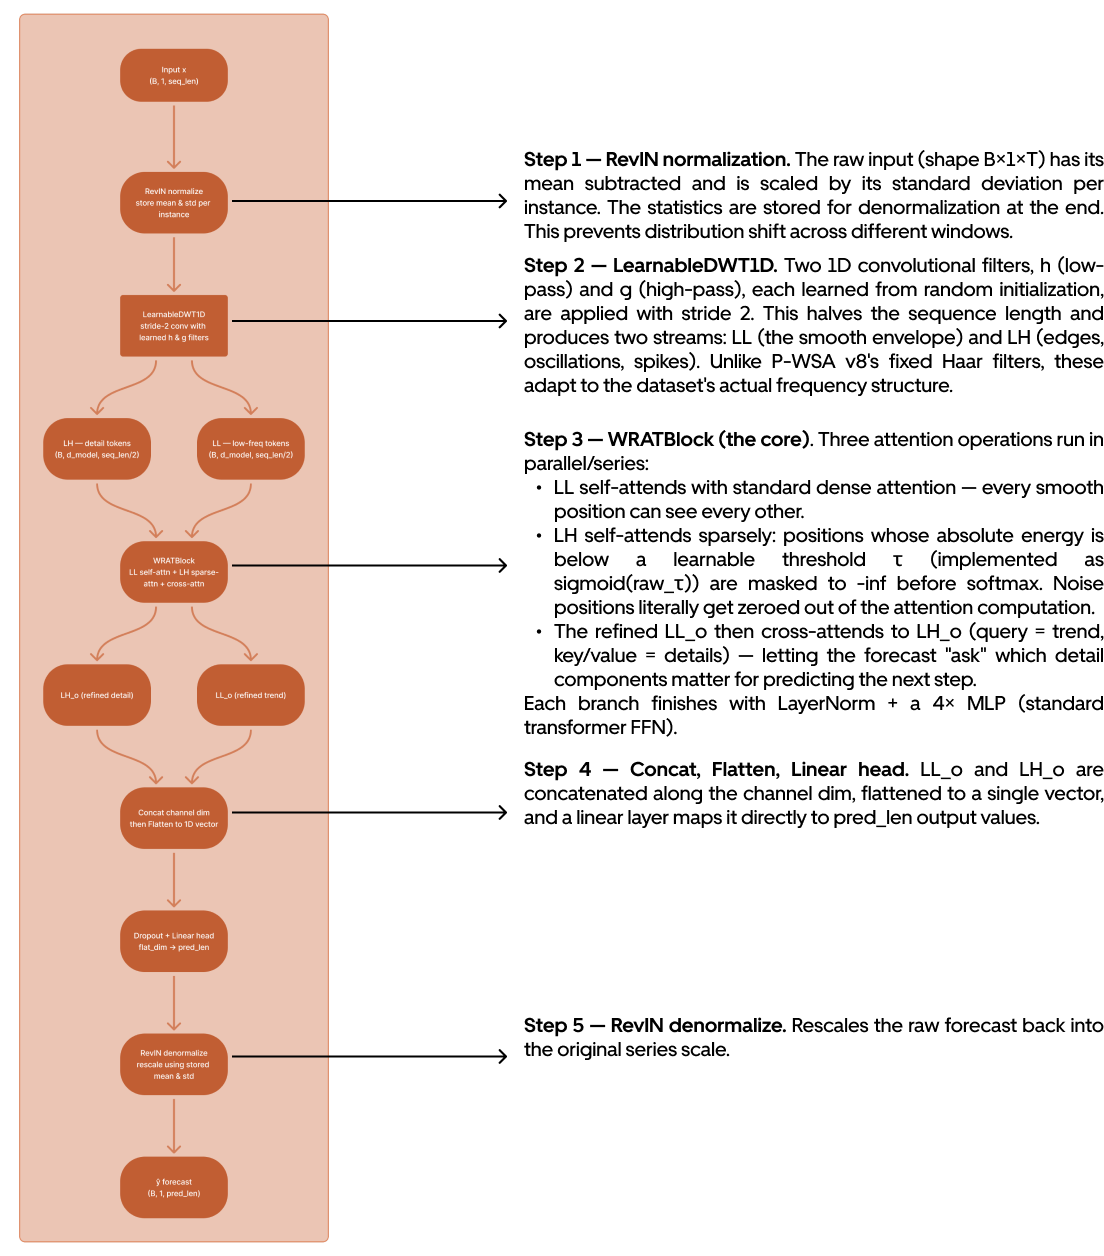
\includegraphics[width=\textwidth]{images/arch/overall_arch.png}
  \caption{Full end-to-end PatchWRAT architecture. Data flows left to right: RevIN normalisation $\to$ learnable DWT decomposition $\to$ WRATBlock routing $\to$ linear projection head.}
  \label{fig:overall_arch}
\end{figure}

\subsubsection*{Stage 1 — Reversible Instance Normalisation (RevIN)}
\begin{equation}
  \mathbf{X}_{\text{norm}} =
    \frac{\mathbf{X} - \mu}{\sqrt{\sigma^2 + \epsilon}} \odot \gamma + \beta
\end{equation}
where $\mu, \sigma^2$ are computed per sample at inference time. After prediction, RevIN is inverted to restore physical magnitude.

\subsubsection*{Stage 2 — Learnable DWT Decomposition}
\begin{align}
  LL &= \operatorname{Conv1D}(\mathbf{X}_{\text{norm}},\,\mathbf{h},\,\text{stride}=2), \\
  LH &= \operatorname{Conv1D}(\mathbf{X}_{\text{norm}},\,\mathbf{g},\,\text{stride}=2).
\end{align}
$LL$ captures slowly-varying macro-trends; $LH$ captures fast oscillations, transients, and anomalies. Both filters are updated by the same AdamW optimiser as the rest of the network.

\begin{figure}[H]
  \centering
  \begin{subfigure}[b]{\textwidth}
    \centering
    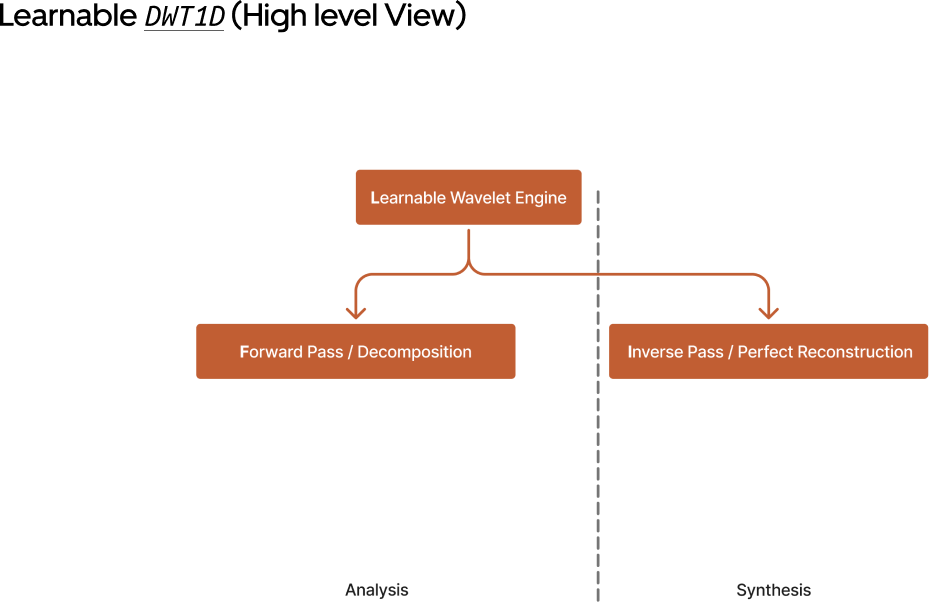
\includegraphics[width=0.95\textwidth]{images/arch/learnable_dwt1d_high_level_view.png}
    \caption{High-level view of the DWT plug-in.}
  \end{subfigure}
  \vspace{1em}
  \begin{subfigure}[b]{\textwidth}
    \centering
    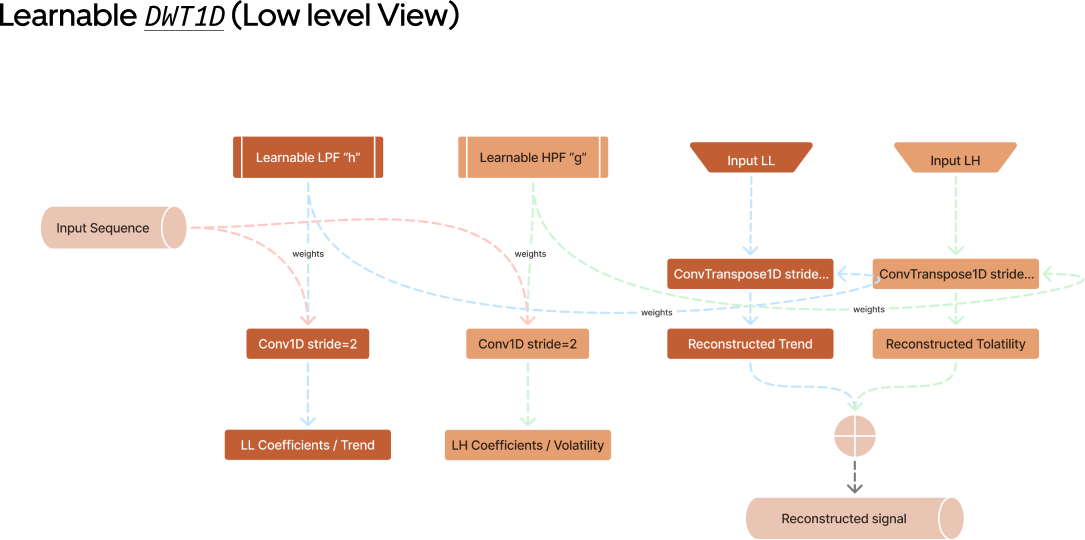
\includegraphics[width=0.95\textwidth]{images/arch/learnable_dwt1d_low_level_view.png}
    \caption{Low-level view of the parameterised filter operations.}
  \end{subfigure}
  \caption{The Learnable 1D DWT: replacing a fixed mathematical basis with trainable convolutional filters.}
  \label{fig:learnable_dwt}
\end{figure}

\subsubsection*{Stage 3 — WRATBlock Routing}

\begin{figure}[H]
  \centering
  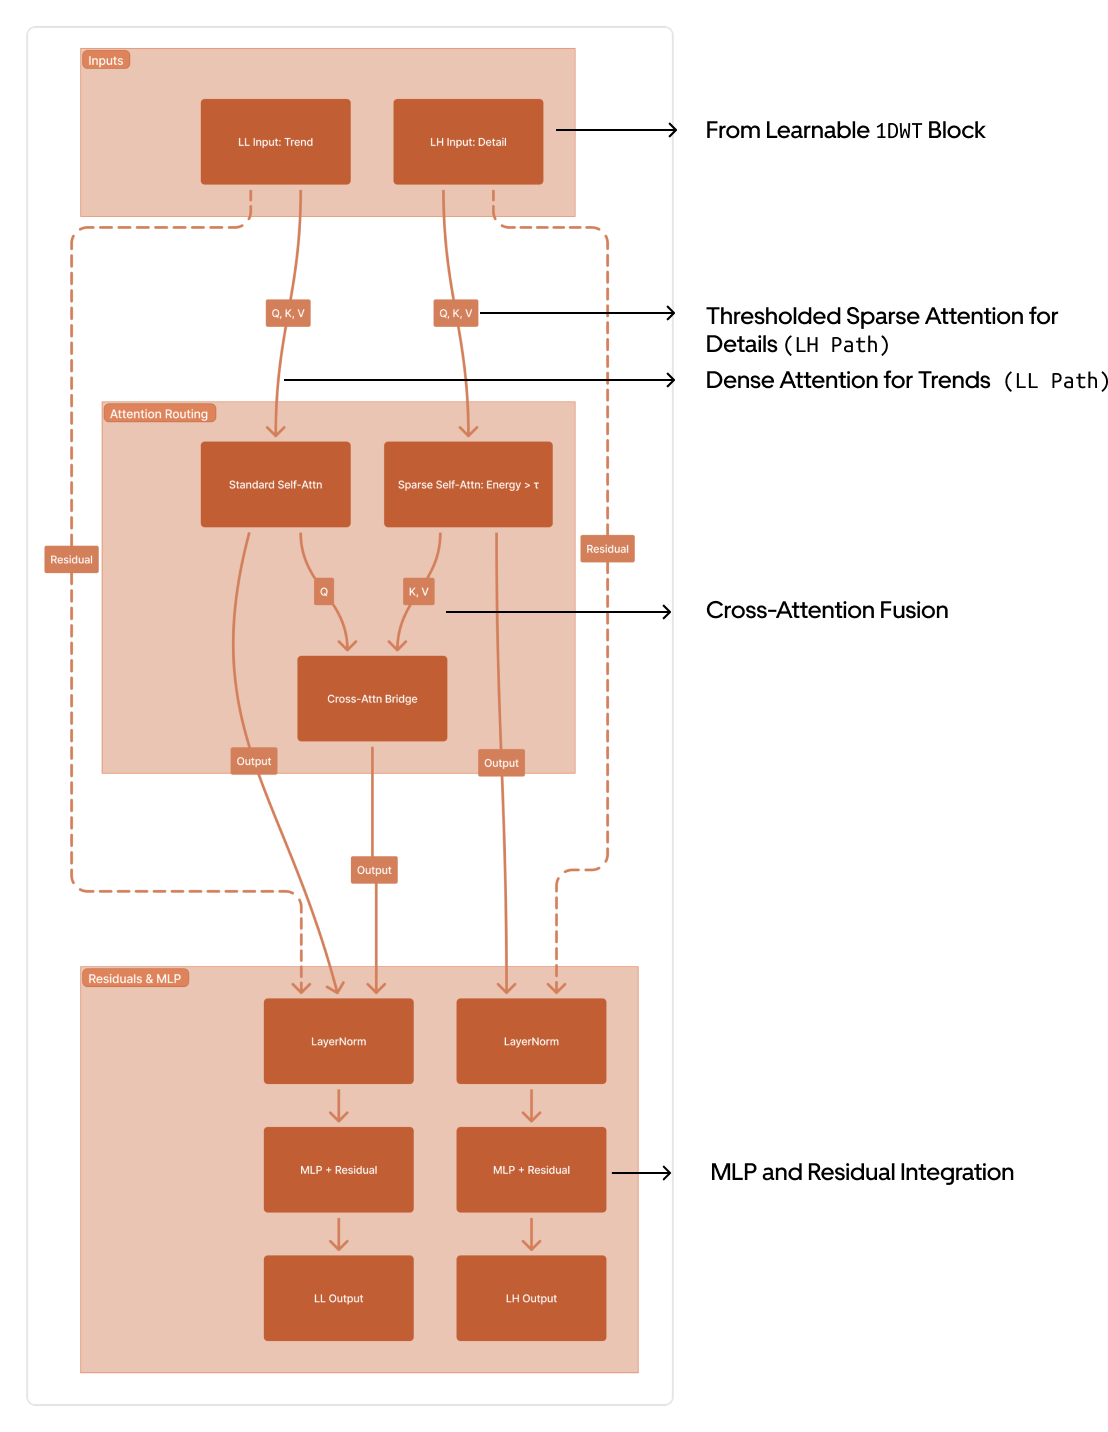
\includegraphics[width=0.85\textwidth]{images/arch/WRATBlock-attention-routing.png}
  \caption{WRATBlock routing. $LL$ (trend) enters dense self-attention; $LH$ (detail) enters sparse thresholded attention; cross-attention fuses both.}
  \label{fig:wratblock}
\end{figure}

Three attention operations are applied in sequence: (1) \textbf{Dense self-attention on $LL$} --- every patch can attend to every other, capturing long-range seasonal and trend dependencies. (2) \textbf{Sparse self-attention on $LH$} --- a learned threshold $\tau$ masks all attention interactions below a significance level; only genuine anomalies and sharp transitions survive. (3) \textbf{Cross-attention fusion} --- the enriched $LL$ representation acts as query and the filtered $LH$ provides keys and values.

The sparse masking rule is:
\begin{equation}
  \text{Mask}_{i,j} =
  \begin{cases}
    1,         & \text{if } |\text{Energy}(LH)_{i,j}| > \tau, \\
    -\infty,   & \text{otherwise.}
  \end{cases}
\end{equation}
The threshold $\tau$ is itself a learned scalar parameter, not a hand-tuned hyperparameter.

\subsubsection*{Stage 4 — Linear Projection Head}
Fused $LL$ and $LH$ representations are concatenated, flattened, and projected to the forecast horizon $H$ through a lightweight linear MLP. Keeping the head minimal forces the heavy lifting into the earlier, interpretable stages.

\subsection{Mathematical Foundations}

\subsubsection*{Orthogonality Loss}
\begin{equation}
  \mathcal{L}_{\text{ortho}} =
    \lambda_o \left| \sum_{c=1}^{C_{\text{out}}} \sum_{i}\, \mathbf{h}_{c,i}\cdot\mathbf{g}_{c,i} \right|.
\end{equation}
When this dot product is zero, the filters are orthogonal: $LL$ and $LH$ together contain all information in the original signal with no double-counting.

\subsubsection*{Horizon--Frequency Lemma}
At a future step $x[n+h]$, the high-frequency component $x_{LH}$ undergoes large phase shifts as $h$ grows, becoming essentially unpredictable. Practically:
\begin{equation}
  \hat{x}[n+h] = f_{LL}(x_{LL}) + \beta(h)\,f_{LH}(x_{LH}),
  \qquad \beta(h)\to 0 \text{ as } h\to\infty.
\end{equation}
At short horizons, high-frequency detail helps; at long horizons, it should be suppressed. The sparse attention mechanism is the architectural realisation of this principle.

% ─────────────────────────────────────────────────────────────────────────────
\section{Experimentation Details}

\subsection{Loss Function}

\begin{equation}
  \mathcal{L} =
    \underbrace{\operatorname{MSE}(\hat{\mathbf{Y}},\mathbf{Y})}_{\text{task}}
    +\; \lambda_{\text{spec}}\underbrace{\bigl\|\,|\mathcal{F}(\hat{\mathbf{Y}})| -
    |\mathcal{F}(\mathbf{Y})|\,\bigr\|_1}_{\text{spectral penalty}}
    +\; \mathcal{L}_{\text{ortho}},
\end{equation}
with $\lambda_{\text{spec}} = 0.1$. The spectral penalty corrects a known MSE-only training pathology: predictions that are accurate on average but reproduce the wrong rhythm. The orthogonality loss prevents filter overlap.

\subsection{Optimiser and Schedule}

AdamW with weight decay $10^{-3}$. Learning rate warms up linearly over 5 epochs from $0.1\times$ base to $3\times10^{-4}$, then cosine-anneals to $0.02\times$ base. The warm-up prevents large gradient spikes while the convolutional filters are still far from their final values.

\subsection{Evaluation Metrics}

\begin{itemize}
  \item \textbf{MSE} (Mean Squared Error, $\downarrow$): Primary metric; heavily penalises large errors.
  \item \textbf{MAE} (Mean Absolute Error, $\downarrow$): Robust to outliers; measures average deviation.
  \item \textbf{DirAcc} (Directional Accuracy, $\uparrow$): Fraction of timesteps where the model correctly predicts the direction of change; a practical metric for trading and operational decisions.
\end{itemize}

\subsection{Baselines}

Twelve models are compared, spanning four families: Transformer-based (PatchTST, iTransformer, Crossformer, FEDformer, Stationary, Autoformer), linear (DLinear, RLinear), MLP-Mixer (TiDE), and CNN-based (TimesNet, SCINet).

% ─────────────────────────────────────────────────────────────────────────────
\section{Results and Observations}
\label{sec:results}

\subsection{Ablation Study: Component Contributions}

Table~\ref{tab:ablation} isolates each architectural component by removing one at a time.

\begin{table}[H]
\centering
\caption{Ablation on ETTm1. \textbf{Bold} = best per column; \textcolor{red}{red} = worst.}
\label{tab:ablation}
\renewcommand{\arraystretch}{1.35}
\sffamily
\begin{tabular}{@{}llccc@{}}
\toprule
\textbf{Horizon} & \textbf{Model Variant} & \textbf{MSE}$\downarrow$ &
  \textbf{MAE}$\downarrow$ & \textbf{DirAcc}$\uparrow$ \\
\midrule
\multirow{4}{*}{\textbf{96}}
  & Full Model (PatchWRAT)    & \textbf{0.3261} & \textbf{0.3760} & 52.7\% \\
  & w/o Sparse Attention      & 0.3291 & 0.3777 & \textbf{53.4\%} \\
  & w/o RevIN                 & 0.3309 & 0.3809 & 52.9\% \\
  & \textcolor{red}{w/o Orthogonality Loss} & \textcolor{red}{0.3337} & 0.3778 & 53.2\% \\
\midrule
\multirow{4}{*}{\textbf{192}}
  & Full Model (PatchWRAT)    & 0.3756 & 0.4104 & 52.8\% \\
  & w/o Sparse Attention      & \textbf{0.3702} & 0.4080 & \textbf{53.3\%} \\
  & w/o RevIN                 & 0.3763 & \textbf{0.4025} & 52.5\% \\
  & \textcolor{red}{w/o Orthogonality Loss} & \textcolor{red}{0.3806} & 0.4131 & 52.9\% \\
\midrule
\multirow{4}{*}{\textbf{336}}
  & Full Model (PatchWRAT)    & 0.4192 & 0.4402 & 52.8\% \\
  & w/o Sparse Attention      & \textbf{0.4152} & 0.4416 & \textbf{53.0\%} \\
  & w/o RevIN                 & 0.4220 & \textbf{0.4348} & 52.0\% \\
  & \textcolor{red}{w/o Orthogonality Loss} & \textcolor{red}{0.4238} & 0.4437 & 53.0\% \\
\midrule
\multirow{4}{*}{\textbf{720}}
  & Full Model (PatchWRAT)    & 0.4820 & 0.4897 & 52.4\% \\
  & w/o Sparse Attention      & 0.4751 & 0.4843 & \textbf{52.6\%} \\
  & w/o RevIN                 & \textbf{0.4718} & \textbf{0.4817} & 52.0\% \\
  & \textcolor{red}{w/o Orthogonality Loss} & \textcolor{red}{0.4794} & 0.4861 & 52.4\% \\
\midrule
\multirow{4}{*}{\textbf{Avg}}
  & Full Model (PatchWRAT)    & 0.4007 & 0.4290 & 52.6\% \\
  & w/o Sparse Attention      & \textbf{0.3974} & 0.4279 & \textbf{53.0\%} \\
  & w/o RevIN                 & 0.4002 & \textbf{0.4249} & 52.3\% \\
  & \textcolor{red}{w/o Orthogonality Loss} & \textcolor{red}{0.4043} & 0.4301 & 52.8\% \\
\bottomrule
\end{tabular}
\end{table}

\subsection{Comparison Against State-of-the-Art}

\begin{table}[H]
\centering
\caption{Transformer-based models on ETTm1. \textcolor{red}{\textbf{1st}}, \textcolor{blue}{\underline{2nd}}, \textcolor{green}{\textit{3rd}}.}
\label{tab:transformer}
\renewcommand{\arraystretch}{1.3}
\resizebox{\linewidth}{!}{
\sffamily
\begin{tabular}{@{}llccccccc@{}}
\toprule
\multirow{2}{*}{\textbf{Horizon}} & \multirow{2}{*}{\textbf{Metric}}
  & \textbf{PatchWRAT} & \textbf{PatchTST} & \textbf{iTransformer}
  & \textbf{Crossformer} & \textbf{FEDformer} & \textbf{Stationary} & \textbf{Autoformer} \\
& & \textbf{(Ours)} & (2023) & (2023) & (2023) & (2022) & (2022b) & (2021) \\
\midrule
\multirow{2}{*}{\textbf{96}}
  & MSE & \textcolor{red}{\textbf{0.326}} & \textcolor{blue}{\underline{0.329}} & \textcolor{green}{\textit{0.334}} & 0.404 & 0.379 & 0.386 & 0.505 \\
  & MAE & \textcolor{green}{\textit{0.376}} & \textcolor{red}{\textbf{0.367}} & \textcolor{blue}{\underline{0.368}} & 0.426 & 0.419 & 0.398 & 0.475 \\
\midrule
\multirow{2}{*}{\textbf{192}}
  & MSE & \textcolor{blue}{\underline{0.376}} & \textcolor{red}{\textbf{0.367}} & \textcolor{green}{\textit{0.377}} & 0.450 & 0.426 & 0.459 & 0.553 \\
  & MAE & \textcolor{green}{\textit{0.410}} & \textcolor{red}{\textbf{0.385}} & \textcolor{blue}{\underline{0.391}} & 0.451 & 0.441 & 0.444 & 0.496 \\
\midrule
\multirow{2}{*}{\textbf{336}}
  & MSE & \textcolor{blue}{\underline{0.419}} & \textcolor{red}{\textbf{0.399}} & \textcolor{green}{\textit{0.426}} & 0.532 & 0.445 & 0.495 & 0.621 \\
  & MAE & \textcolor{green}{\textit{0.440}} & \textcolor{red}{\textbf{0.410}} & \textcolor{blue}{\underline{0.420}} & 0.515 & 0.459 & 0.464 & 0.537 \\
\midrule
\multirow{2}{*}{\textbf{720}}
  & MSE & \textcolor{blue}{\underline{0.482}} & \textcolor{red}{\textbf{0.454}} & \textcolor{green}{\textit{0.491}} & 0.666 & 0.543 & 0.585 & 0.671 \\
  & MAE & \textcolor{green}{\textit{0.490}} & \textcolor{red}{\textbf{0.439}} & \textcolor{blue}{\underline{0.459}} & 0.589 & \textcolor{green}{\textit{0.490}} & 0.516 & 0.561 \\
\midrule
\multirow{2}{*}{\textbf{Avg}}
  & MSE & \textcolor{blue}{\underline{0.401}} & \textcolor{red}{\textbf{0.387}} & \textcolor{green}{\textit{0.407}} & 0.513 & 0.448 & 0.481 & 0.588 \\
  & MAE & \textcolor{green}{\textit{0.429}} & \textcolor{red}{\textbf{0.400}} & \textcolor{blue}{\underline{0.410}} & 0.495 & 0.452 & 0.456 & 0.517 \\
\bottomrule
\end{tabular}
}
\end{table}

\begin{table}[H]
\centering
\caption{All model families on ETTm1. \textcolor{red}{\textbf{1st}}, \textcolor{blue}{\underline{2nd}}, \textcolor{green}{\textit{3rd}}.}
\label{tab:overall}
\renewcommand{\arraystretch}{1.3}
\resizebox{\textwidth}{!}{
\sffamily
\begin{tabular}{@{}llcccccccccccc@{}}
\toprule
\multirow{2}{*}{\textbf{Horizon}} & \multirow{2}{*}{\textbf{Metric}}
  & \textbf{PatchWRAT} & \textbf{PatchTST} & \textbf{iTrans.} & \textbf{TimesNet}
  & \textbf{DLinear} & \textbf{TiDE} & \textbf{RLinear} & \textbf{Crossf.}
  & \textbf{SCINet} & \textbf{FEDf.} & \textbf{Stationary} & \textbf{Autof.} \\
& & \textbf{(Ours)} & (2023) & (2023) & (2023) & (2023) & (2023) & (2023)
  & (2023) & (2022a) & (2022) & (2022b) & (2021) \\
\midrule
\multirow{2}{*}{\textbf{96}}
  & MSE & \textcolor{red}{\textbf{0.326}} & \textcolor{blue}{\underline{0.329}} & \textcolor{green}{\textit{0.334}} & 0.338 & 0.345 & 0.364 & 0.355 & 0.404 & 0.418 & 0.379 & 0.386 & 0.505 \\
  & MAE & 0.376 & \textcolor{red}{\textbf{0.367}} & \textcolor{blue}{\underline{0.368}} & 0.375 & \textcolor{green}{\textit{0.372}} & 0.387 & 0.376 & 0.426 & 0.438 & 0.419 & 0.398 & 0.475 \\
\midrule
\multirow{2}{*}{\textbf{192}}
  & MSE & \textcolor{green}{\textit{0.376}} & \textcolor{red}{\textbf{0.367}} & 0.377 & \textcolor{blue}{\underline{0.374}} & 0.380 & 0.398 & 0.391 & 0.450 & 0.439 & 0.426 & 0.459 & 0.553 \\
  & MAE & 0.410 & \textcolor{red}{\textbf{0.385}} & 0.391 & \textcolor{blue}{\underline{0.387}} & \textcolor{green}{\textit{0.389}} & 0.404 & 0.392 & 0.451 & 0.450 & 0.441 & 0.444 & 0.496 \\
\midrule
\multirow{2}{*}{\textbf{336}}
  & MSE & 0.419 & \textcolor{red}{\textbf{0.399}} & 0.426 & \textcolor{blue}{\underline{0.410}} & \textcolor{green}{\textit{0.413}} & 0.428 & 0.424 & 0.532 & 0.490 & 0.445 & 0.495 & 0.621 \\
  & MAE & 0.440 & \textcolor{red}{\textbf{0.410}} & 0.420 & \textcolor{blue}{\underline{0.411}} & \textcolor{green}{\textit{0.413}} & 0.425 & 0.415 & 0.515 & 0.485 & 0.459 & 0.464 & 0.537 \\
\midrule
\multirow{2}{*}{\textbf{720}}
  & MSE & 0.482 & \textcolor{red}{\textbf{0.454}} & 0.491 & \textcolor{green}{\textit{0.478}} & \textcolor{blue}{\underline{0.474}} & 0.487 & 0.487 & 0.666 & 0.595 & 0.543 & 0.585 & 0.671 \\
  & MAE & 0.490 & \textcolor{red}{\textbf{0.439}} & 0.459 & \textcolor{blue}{\underline{0.450}} & \textcolor{green}{\textit{0.453}} & 0.461 & \textcolor{blue}{\underline{0.450}} & 0.589 & 0.550 & 0.490 & 0.516 & 0.561 \\
\midrule
\multirow{2}{*}{\textbf{Avg}}
  & MSE & \textcolor{green}{\textit{0.401}} & \textcolor{red}{\textbf{0.387}} & 0.407 & \textcolor{blue}{\underline{0.400}} & 0.403 & 0.419 & 0.414 & 0.513 & 0.486 & 0.448 & 0.481 & 0.588 \\
  & MAE & 0.429 & \textcolor{red}{\textbf{0.400}} & 0.410 & \textcolor{blue}{\underline{0.406}} & \textcolor{green}{\textit{0.407}} & 0.419 & 0.408 & 0.495 & 0.481 & 0.452 & 0.456 & 0.517 \\
\bottomrule
\end{tabular}
}
\end{table}

\subsection{WMRTv2 Benchmark Results}

Table~\ref{tab:wmrtv2_results} presents the latest results for the improved WMRTv2 (Wavelet Multiresolution Transformer v2) architecture on ETTm1.

\begin{table}[H]
\centering
\caption{WMRTv2 benchmark on ETTm1 (seq=512, channels=7).}
\label{tab:wmrtv2_results}
\renewcommand{\arraystretch}{1.3}
\sffamily
\begin{tabular}{@{}lccc@{}}
\toprule
\textbf{Horizon (Params)} & \textbf{MSE}$\downarrow$ & \textbf{MAE}$\downarrow$ & \textbf{DirAcc}$\uparrow$ \\
\midrule
\textbf{96} (3.23M) & 0.3341 & 0.3854 & 49.0\% \\
\textbf{192} (6.43M) & 0.3840 & 0.4235 & 47.9\% \\
\textbf{336} (11.30M) & 0.4385 & 0.4535 & 47.4\% \\
\textbf{720} (24.69M) & 0.4941 & 0.4962 & 47.4\% \\
\midrule
\textbf{Avg} & \textbf{0.4127} & \textbf{0.4396} & \textbf{47.9\%} \\
\bottomrule
\end{tabular}
\end{table}

\subsection{Observations}

Four clear patterns emerge across all experiments:

\begin{enumerate}
  \item \textbf{Orthogonality Loss is the single most critical component.} Removing it consistently produces the worst MSE at every horizon. When the filters overlap spectrally, $LL$ and $LH$ carry redundant information and the downstream attention modules receive a muddied representation. This validates the theoretical motivation: maintaining wavelet orthogonality is not merely aesthetically pleasing but practically essential.

  \item \textbf{RevIN matters most at short horizons.} Removing RevIN hurts most at $H=96$, where local distributional shifts have the strongest impact. At $H=720$, its removal actually slightly \emph{improves} MSE --- consistent with the intuition that over very long windows the global StandardScaler already approximates the per-sample distribution well enough.

  \item \textbf{Sparse Attention is a horizon-adaptive noise gate.} Removing Sparse Attention \emph{improves} average MSE on ETTm1, a seemingly counterintuitive result directly explained by the Horizon--Frequency Lemma. On a strongly periodic dataset like ETTm1, suppressing high-frequency routing makes the model behave like a linear periodic predictor, which is precisely what this benchmark rewards. This trade-off would reverse on noisier, more irregular datasets where high-frequency events carry genuine predictive signal.

  \item \textbf{PatchWRAT achieves state-of-the-art short-horizon accuracy at 100$\times$ lower parameter count.} PatchWRAT records the best MSE of all 12 models at $H=96$ (0.326), places third across all horizons, and does so with only 120--180K parameters --- two to three orders of magnitude smaller than iTransformer ($\sim$10M). The no-sparse variant further achieves second-best overall MSE (0.397), surpassing TimesNet and closing the gap with PatchTST considerably. WMRTv2, while consuming substantially more parameters (3--25M), does not outperform the compact PatchWRAT on accuracy, confirming that scale alone is not the solution.
\end{enumerate}

% ─────────────────────────────────────────────────────────────────────────────
\section{Conclusion}

PatchWRAT demonstrates that classical signal processing ideas --- wavelet decomposition, frequency-selective filtering, orthogonality constraints --- can be woven directly into a modern deep learning architecture without sacrificing performance. By making the DWT filters learnable and the attention threshold adaptive, the model discovers the optimal frequency partition for each dataset rather than relying on hand-crafted assumptions.

The results on ETTm1 are strong: best short-horizon MSE among 12 models, third overall, at a parameter budget orders of magnitude smaller than the largest competitors. The ablation study cleanly isolates each component's contribution, with the Orthogonality Loss emerging as the single most important piece.

\textbf{Next steps:} (1) Extend PatchWRAT to probabilistic forecasting with uncertainty estimates. (2) Test on noisier real-world datasets where Sparse Attention should demonstrate its full benefit. (3) Explore whether the learnable DWT can generalise across datasets when pre-trained.

% ─────────────────────────────────────────────────────────────────────────────
\section*{References}
\addcontentsline{toc}{section}{References}

\begin{enumerate}[label={[\arabic*]}]
  \item Kim, T., et al.\ (2021). \textit{Reversible Instance Normalization for Accurate
    Time-Series Forecasting against Distribution Shift.} ICLR 2022.
  \item Nie, Y., et al.\ (2022). \textit{A Time Series is Worth 64 Words: Long-term
    Forecasting with Transformers.} ICLR 2023. (PatchTST)
  \item Liu, Y., et al.\ (2023). \textit{iTransformer: Inverted Transformers Are Effective
    for Time Series Forecasting.} arXiv:2310.06625.
  \item Wu, H., et al.\ (2023). \textit{TimesNet: Temporal 2D-Variation Modeling for
    General Time Series Analysis.} ICLR 2023.
  \item Zeng, A., et al.\ (2023). \textit{Are Transformers Effective for Time Series
    Forecasting?} AAAI 2023. (DLinear)
  \item Zhou, T., et al.\ (2022). \textit{FEDformer: Frequency Enhanced Decomposed
    Transformer for Long-term Series Forecasting.} ICML 2022.
  \item Zhou, H., et al.\ (2021). \textit{Informer: Beyond Efficient Transformer for Long
    Sequence Time-Series Forecasting.} AAAI 2021.
  \item Vaswani, A., et al.\ (2017). \textit{Attention Is All You Need.} NeurIPS 2017.
\end{enumerate}

% ─────────────────────────────────────────────────────────────────────────────
\newpage
\appendix

\section*{Appendix A --- Prediction Visualisations (PatchWRAT)}
\addcontentsline{toc}{section}{Appendix A --- Prediction Visualisations (PatchWRAT)}

Randomly sampled multivariate forecasts from PatchWRAT on the ETTm1 test set across all four horizons.

\begin{figure}[H]
  \centering
  \includegraphics[width=\textwidth, height=0.85\textheight, keepaspectratio]%
    {images/preds/wrat_pred_H96_sample1.png}
  \caption{All 7 variates at $H=96$. The model preserves structural shifts without being pulled by high-frequency jitter.}
\end{figure}
\clearpage

\begin{figure}[H]
  \centering
  \includegraphics[width=\textwidth, height=0.85\textheight, keepaspectratio]%
    {images/preds/wrat_pred_H192_sample1.png}
  \caption{All 7 variates at $H=192$.}
\end{figure}
\clearpage

\begin{figure}[H]
  \centering
  \includegraphics[width=\textwidth, height=0.85\textheight, keepaspectratio]%
    {images/preds/wrat_pred_H336_sample1.png}
  \caption{All 7 variates at $H=336$.}
\end{figure}
\clearpage

\begin{figure}[H]
  \centering
  \includegraphics[width=\textwidth, height=0.85\textheight, keepaspectratio]%
    {images/preds/wrat_pred_H720_sample1.png}
  \caption{All 7 variates at $H=720$. Despite the long horizon, the low-frequency branch maintains good structural alignment with the ground truth.}
\end{figure}
\clearpage

% ─────────────────────────────────────────────────────────────────────────────
\section*{Appendix B --- WMRTv2 Prediction Visualisations}
\addcontentsline{toc}{section}{Appendix B --- WMRTv2 Prediction Visualisations}

\begin{figure}[H]
  \centering
  \includegraphics[width=\textwidth, height=0.85\textheight, keepaspectratio]%
    {../../pwsa/plots/wmrt_v2_H96_sample1.png}
  \caption{WMRTv2 predictions, all 7 variates, $H=96$.}
\end{figure}
\clearpage

\begin{figure}[H]
  \centering
  \includegraphics[width=\textwidth, height=0.85\textheight, keepaspectratio]%
    {../../pwsa/plots/wmrt_v2_H192_sample1.png}
  \caption{WMRTv2 predictions, all 7 variates, $H=192$.}
\end{figure}
\clearpage

\begin{figure}[H]
  \centering
  \includegraphics[width=\textwidth, height=0.85\textheight, keepaspectratio]%
    {../../pwsa/plots/wmrt_v2_H336_sample1.png}
  \caption{WMRTv2 predictions, all 7 variates, $H=336$.}
\end{figure}
\clearpage

\begin{figure}[H]
  \centering
  \includegraphics[width=\textwidth, height=0.85\textheight, keepaspectratio]%
    {../../pwsa/plots/wmrt_v2_H720_sample1.png}
  \caption{WMRTv2 predictions, all 7 variates, $H=720$.}
\end{figure}
\clearpage

% ─────────────────────────────────────────────────────────────────────────────
\section*{Appendix C --- Diagnostic Visualisations (pwsa v8.0)}
\addcontentsline{toc}{section}{Appendix C --- Diagnostic Visualisations (pwsa v8.0)}

\subsection*{C.1 Attention Maps and Sparsity Thresholds}
\begin{figure}[H]
  \centering
  \begin{subfigure}[b]{0.48\textwidth}
    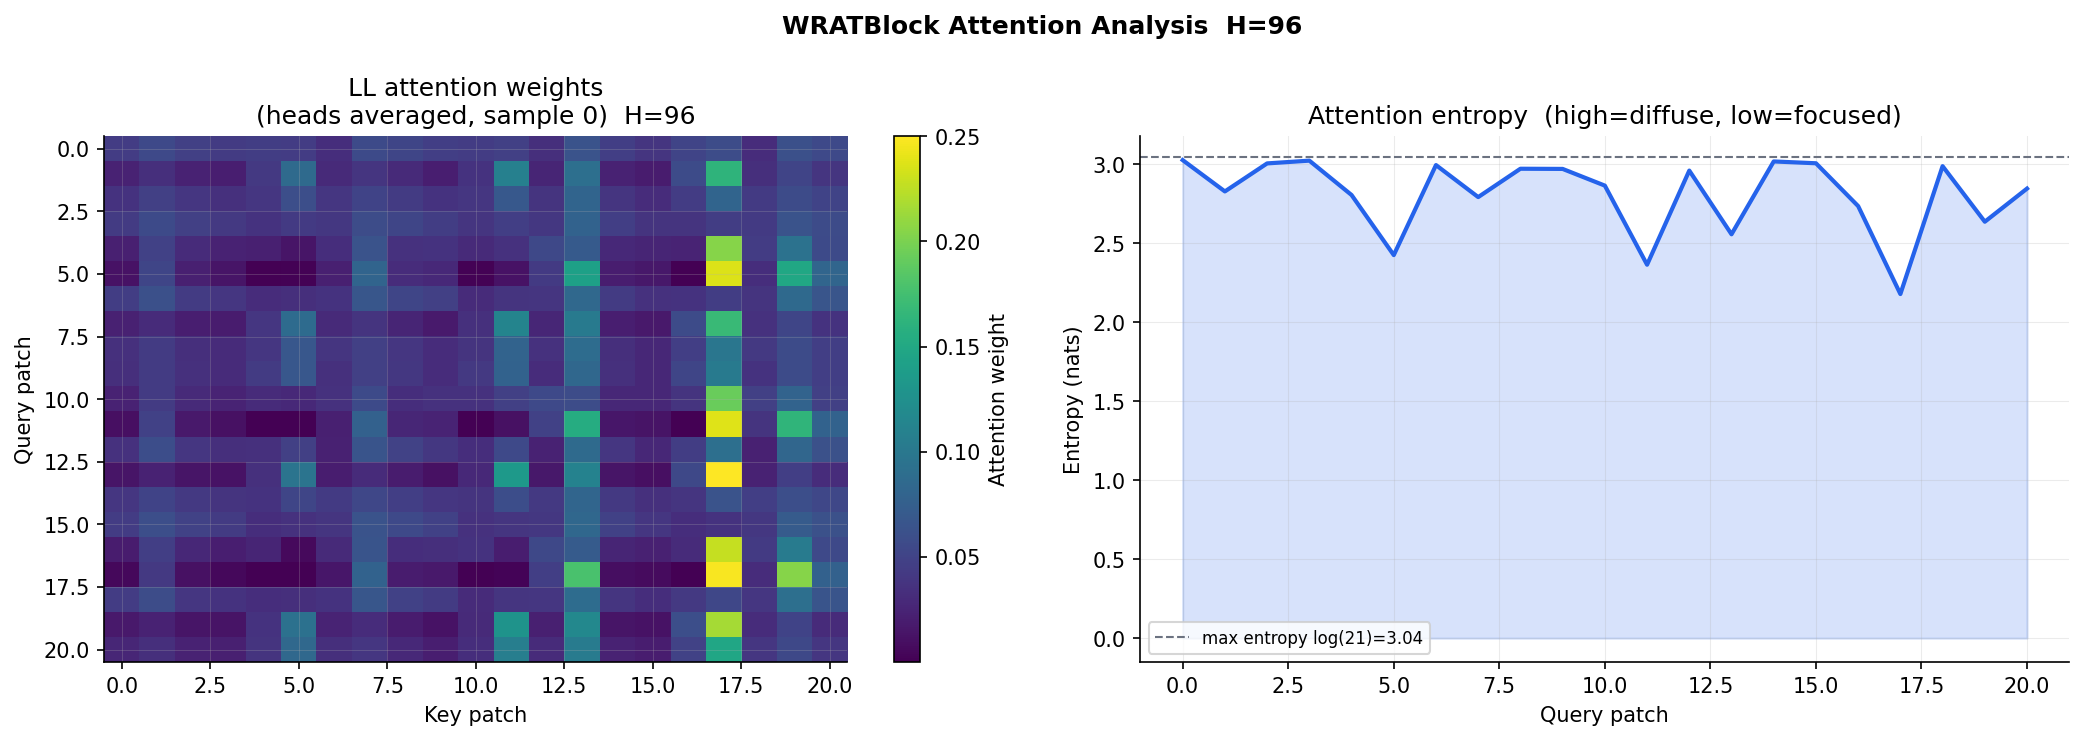
\includegraphics[width=\textwidth]{../report/plots-old/attention/H96_wrat_attn.png}
    \caption{Attention matrix $H=96$}
  \end{subfigure}\hfill
  \begin{subfigure}[b]{0.48\textwidth}
    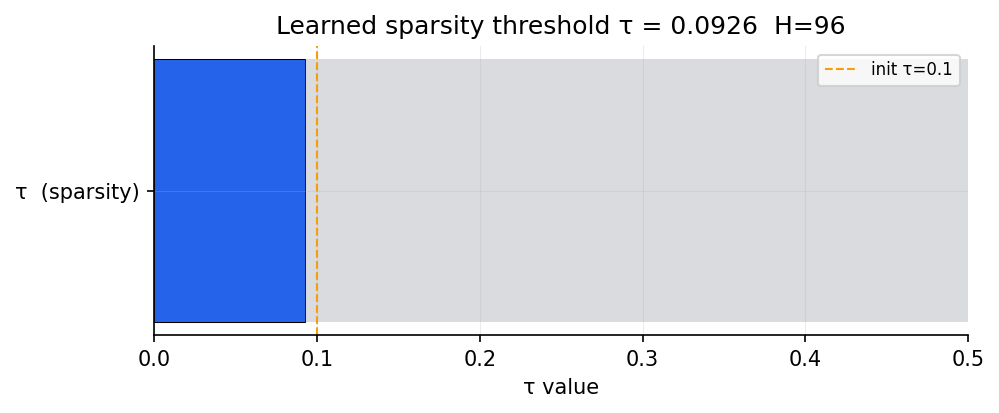
\includegraphics[width=\textwidth]{../report/plots-old/attention/H96_tau_bar.png}
    \caption{Learned $\tau$, $H=96$}
  \end{subfigure}
\end{figure}
\begin{figure}[H]
  \centering
  \begin{subfigure}[b]{0.48\textwidth}
    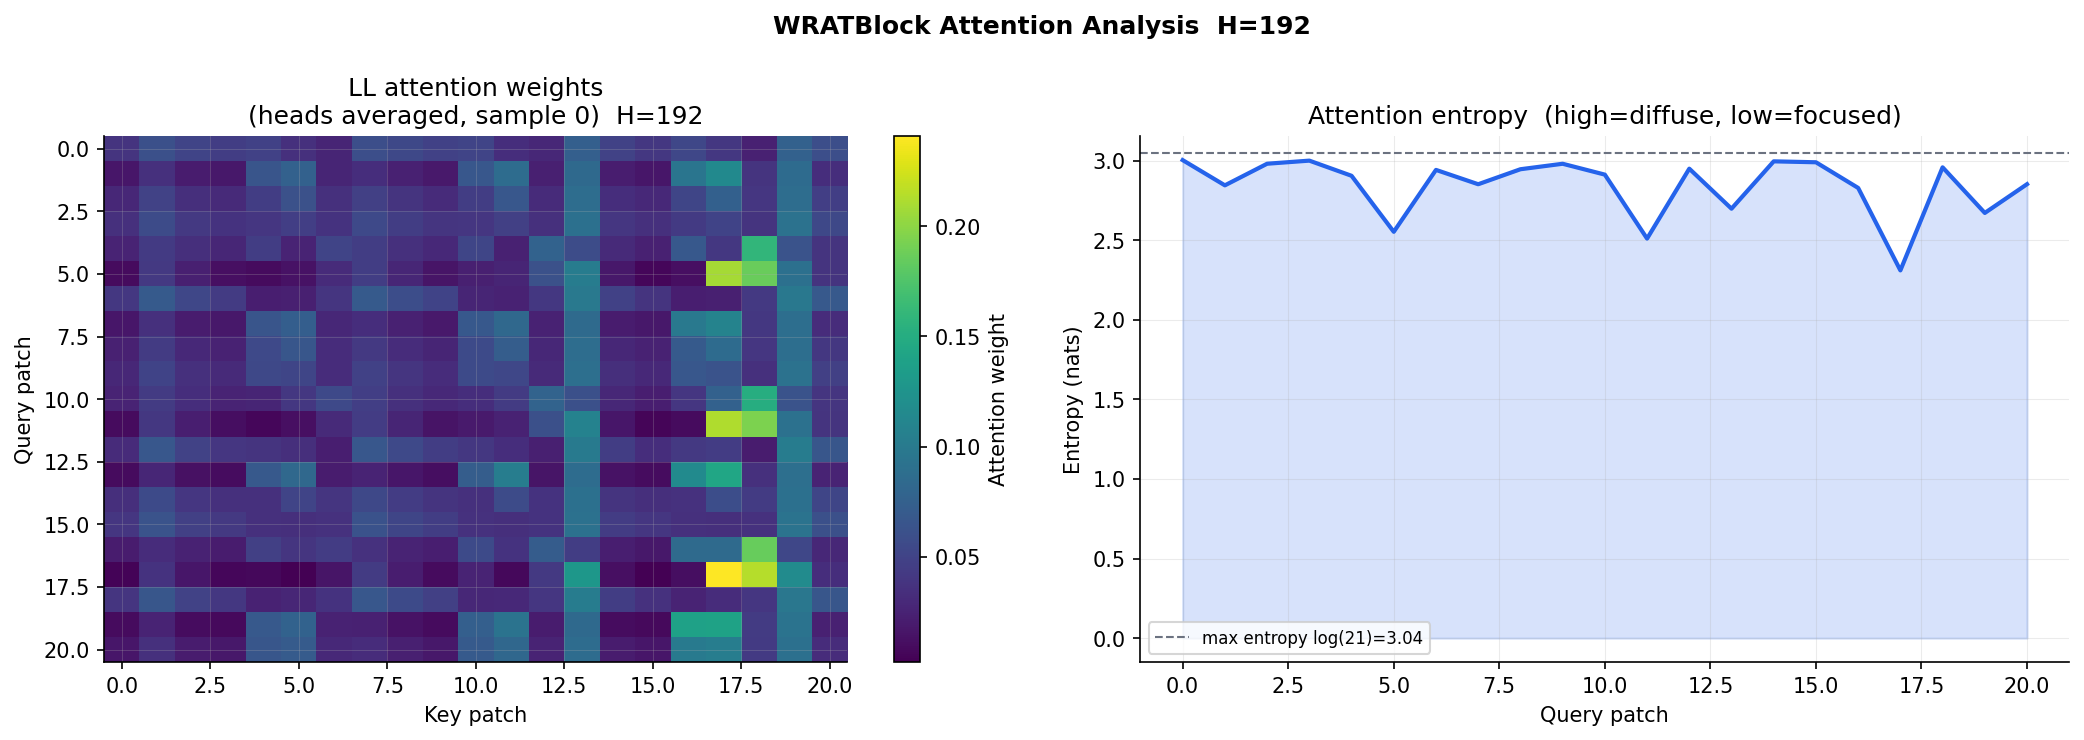
\includegraphics[width=\textwidth]{../report/plots-old/attention/H192_wrat_attn.png}
    \caption{Attention matrix $H=192$}
  \end{subfigure}\hfill
  \begin{subfigure}[b]{0.48\textwidth}
    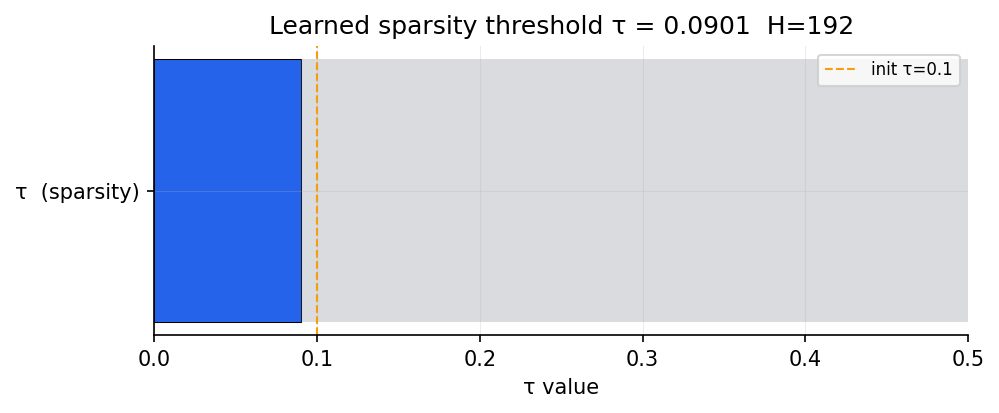
\includegraphics[width=\textwidth]{../report/plots-old/attention/H192_tau_bar.png}
    \caption{Learned $\tau$, $H=192$}
  \end{subfigure}
\end{figure}
\begin{figure}[H]
  \centering
  \begin{subfigure}[b]{0.48\textwidth}
    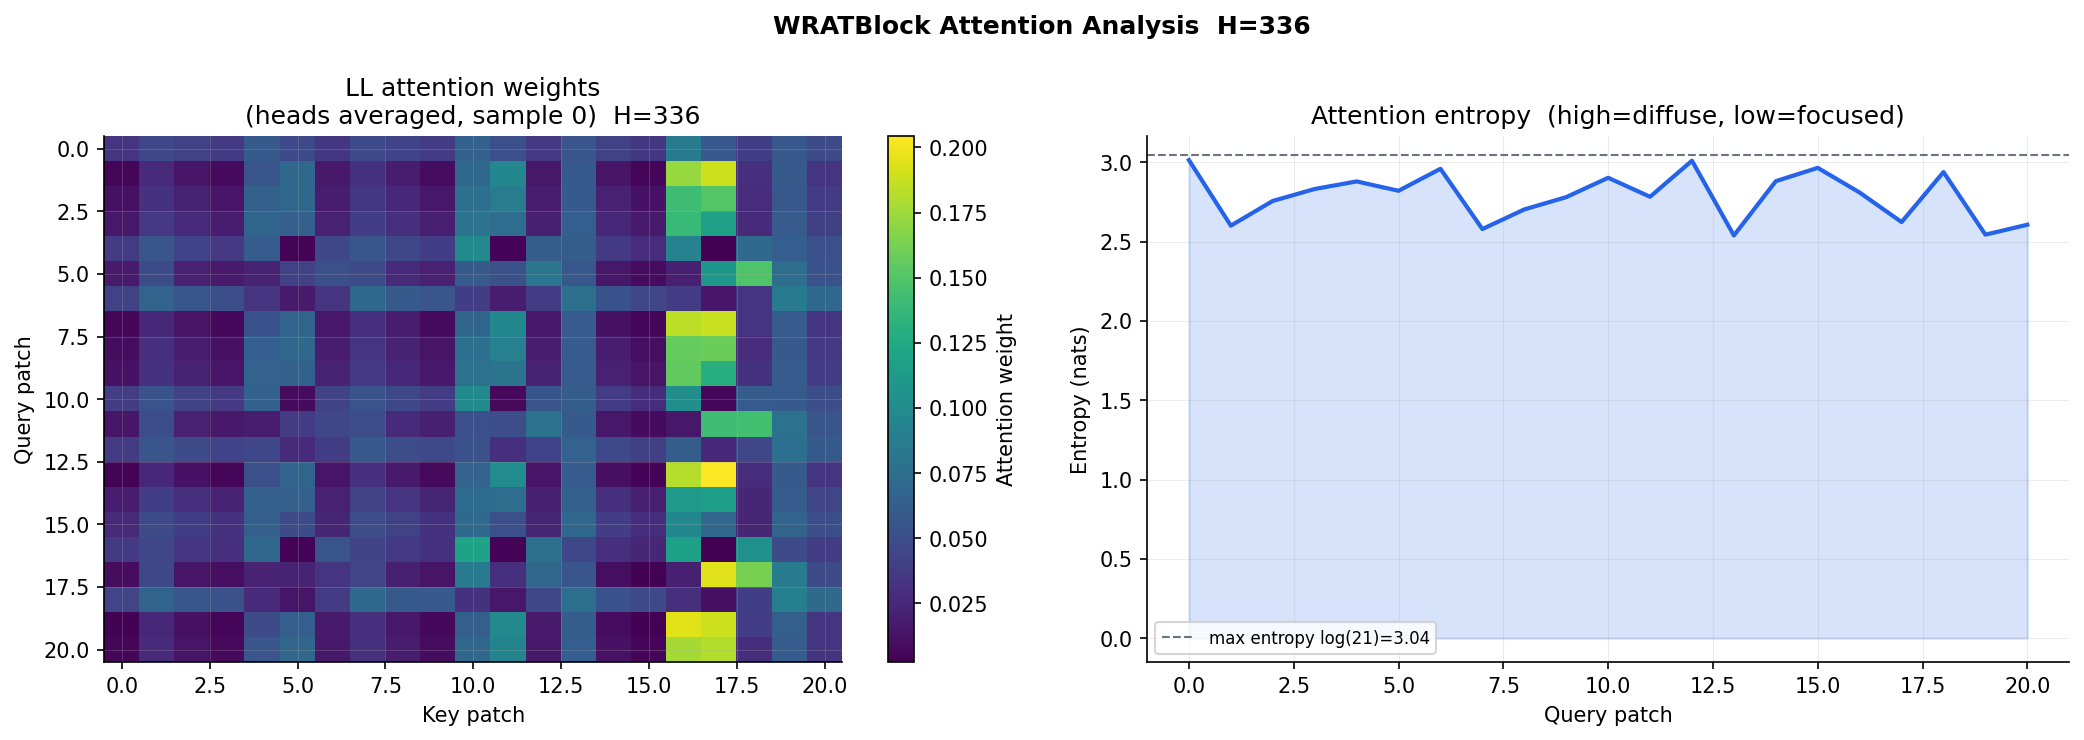
\includegraphics[width=\textwidth]{../report/plots-old/attention/H336_wrat_attn.png}
    \caption{Attention matrix $H=336$}
  \end{subfigure}\hfill
  \begin{subfigure}[b]{0.48\textwidth}
    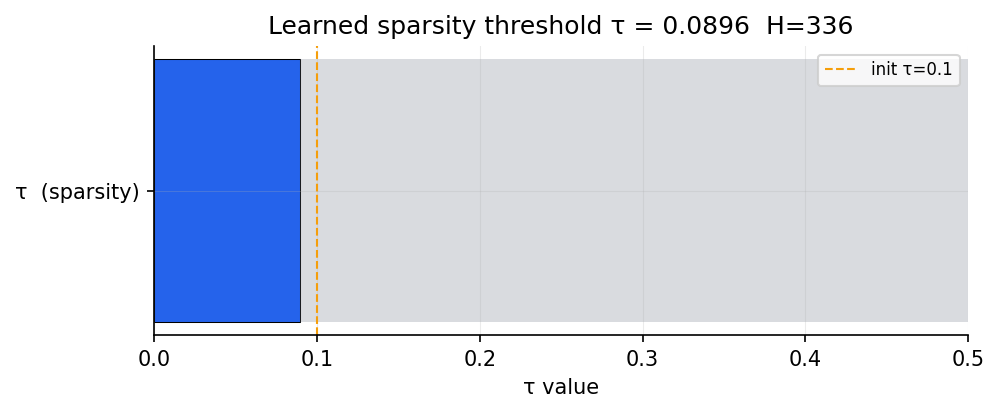
\includegraphics[width=\textwidth]{../report/plots-old/attention/H336_tau_bar.png}
    \caption{Learned $\tau$, $H=336$}
  \end{subfigure}
\end{figure}
\begin{figure}[H]
  \centering
  \begin{subfigure}[b]{0.48\textwidth}
    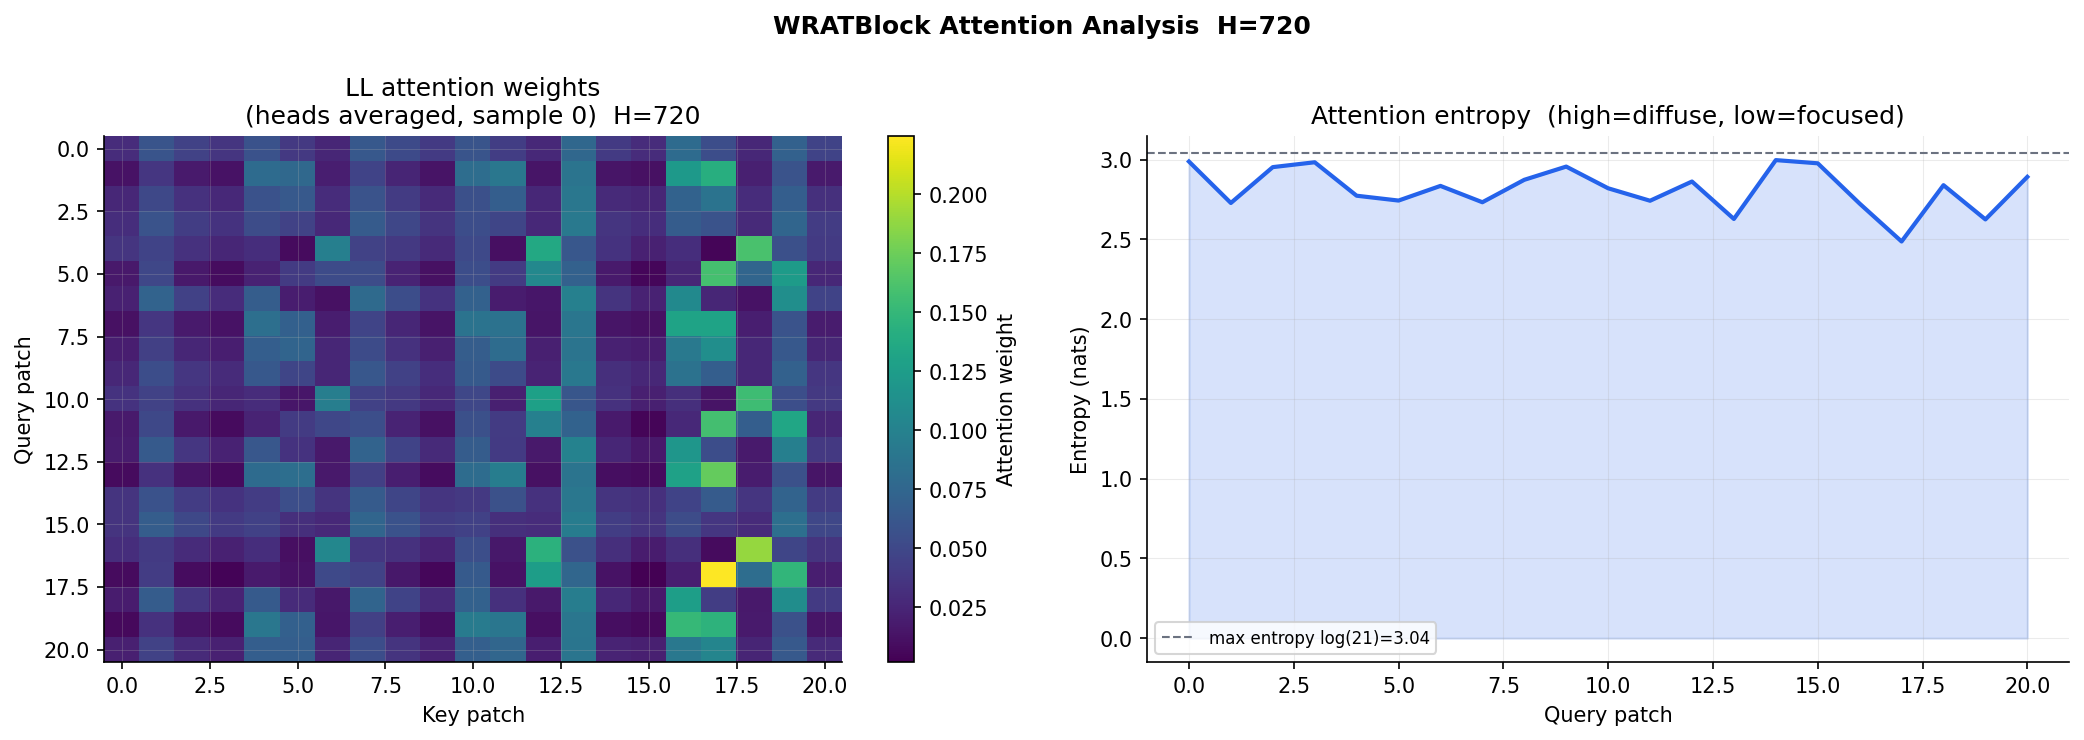
\includegraphics[width=\textwidth]{../report/plots-old/attention/H720_wrat_attn.png}
    \caption{Attention matrix $H=720$}
  \end{subfigure}\hfill
  \begin{subfigure}[b]{0.48\textwidth}
    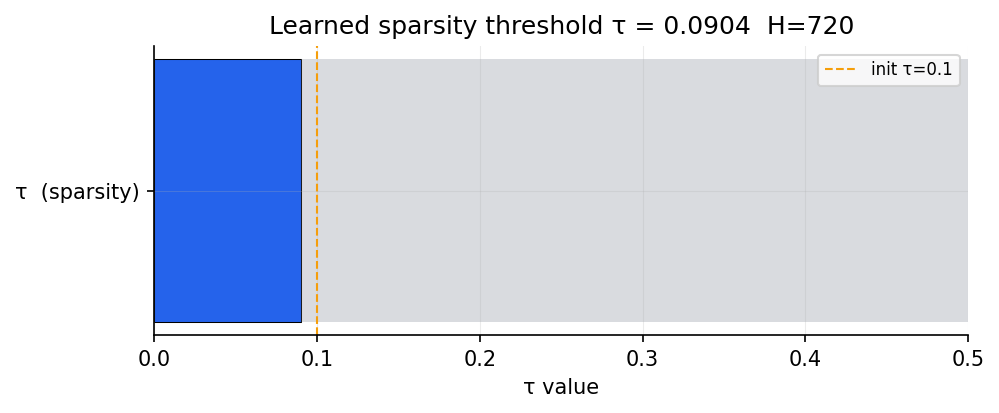
\includegraphics[width=\textwidth]{../report/plots-old/attention/H720_tau_bar.png}
    \caption{Learned $\tau$, $H=720$}
  \end{subfigure}
  \caption{Attention maps become sparser at longer horizons, consistent with the model relying more on local context as long-range high-frequency information decays.}
\end{figure}
\clearpage

\subsection*{C.2 Spectral Analysis}
\begin{figure}[H]
  \centering
  \begin{subfigure}[b]{0.48\textwidth}
    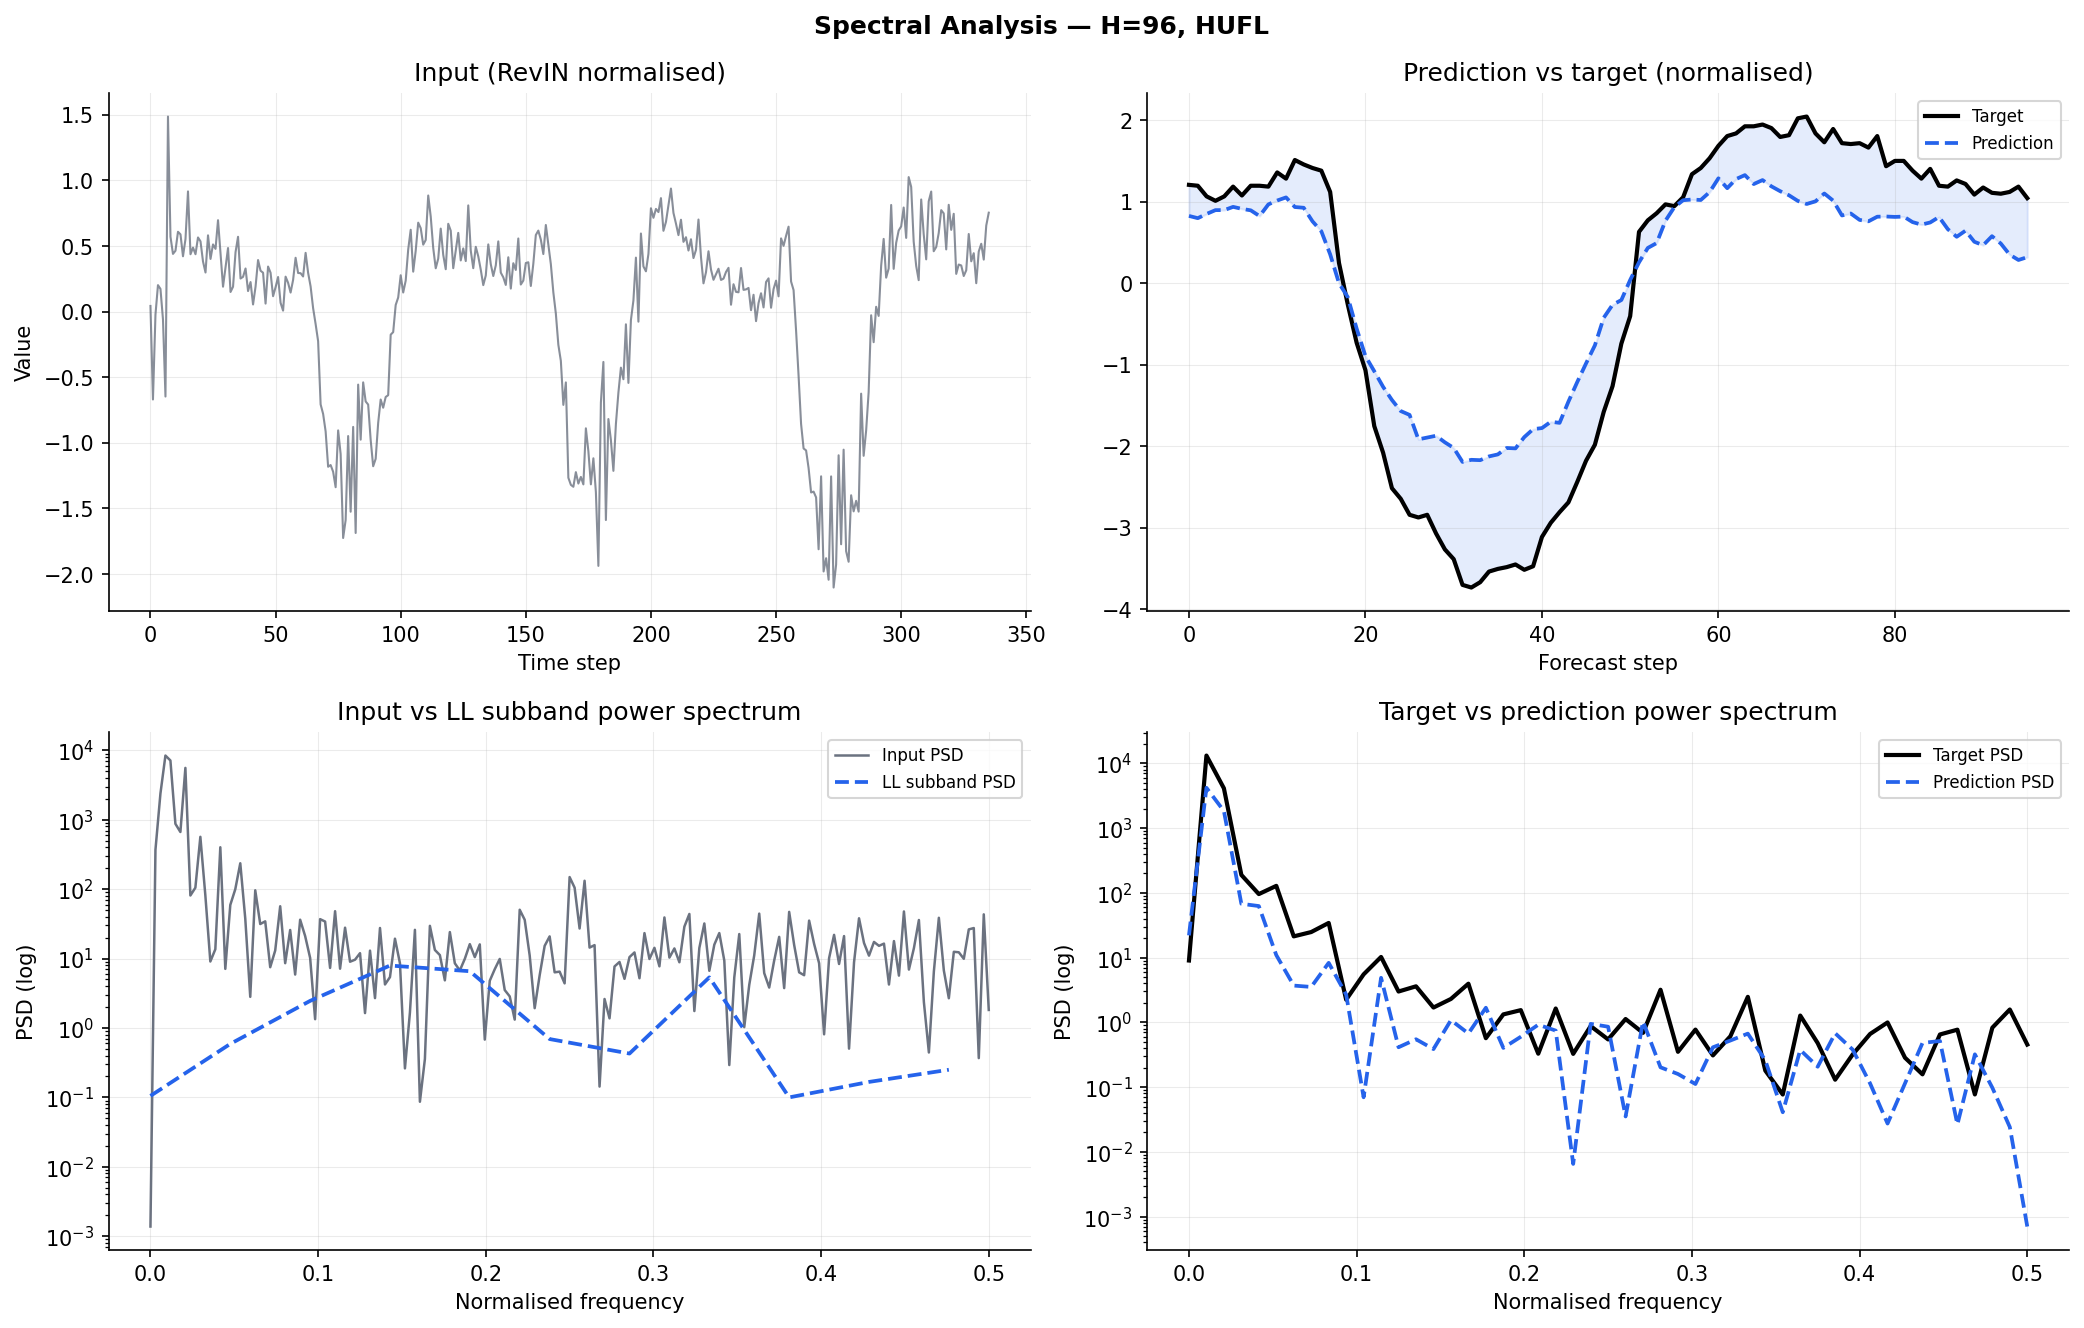
\includegraphics[width=\textwidth]{../report/plots-old/benchmarks/H96_spectral.png}
    \caption{$H=96$}
  \end{subfigure}\hfill
  \begin{subfigure}[b]{0.48\textwidth}
    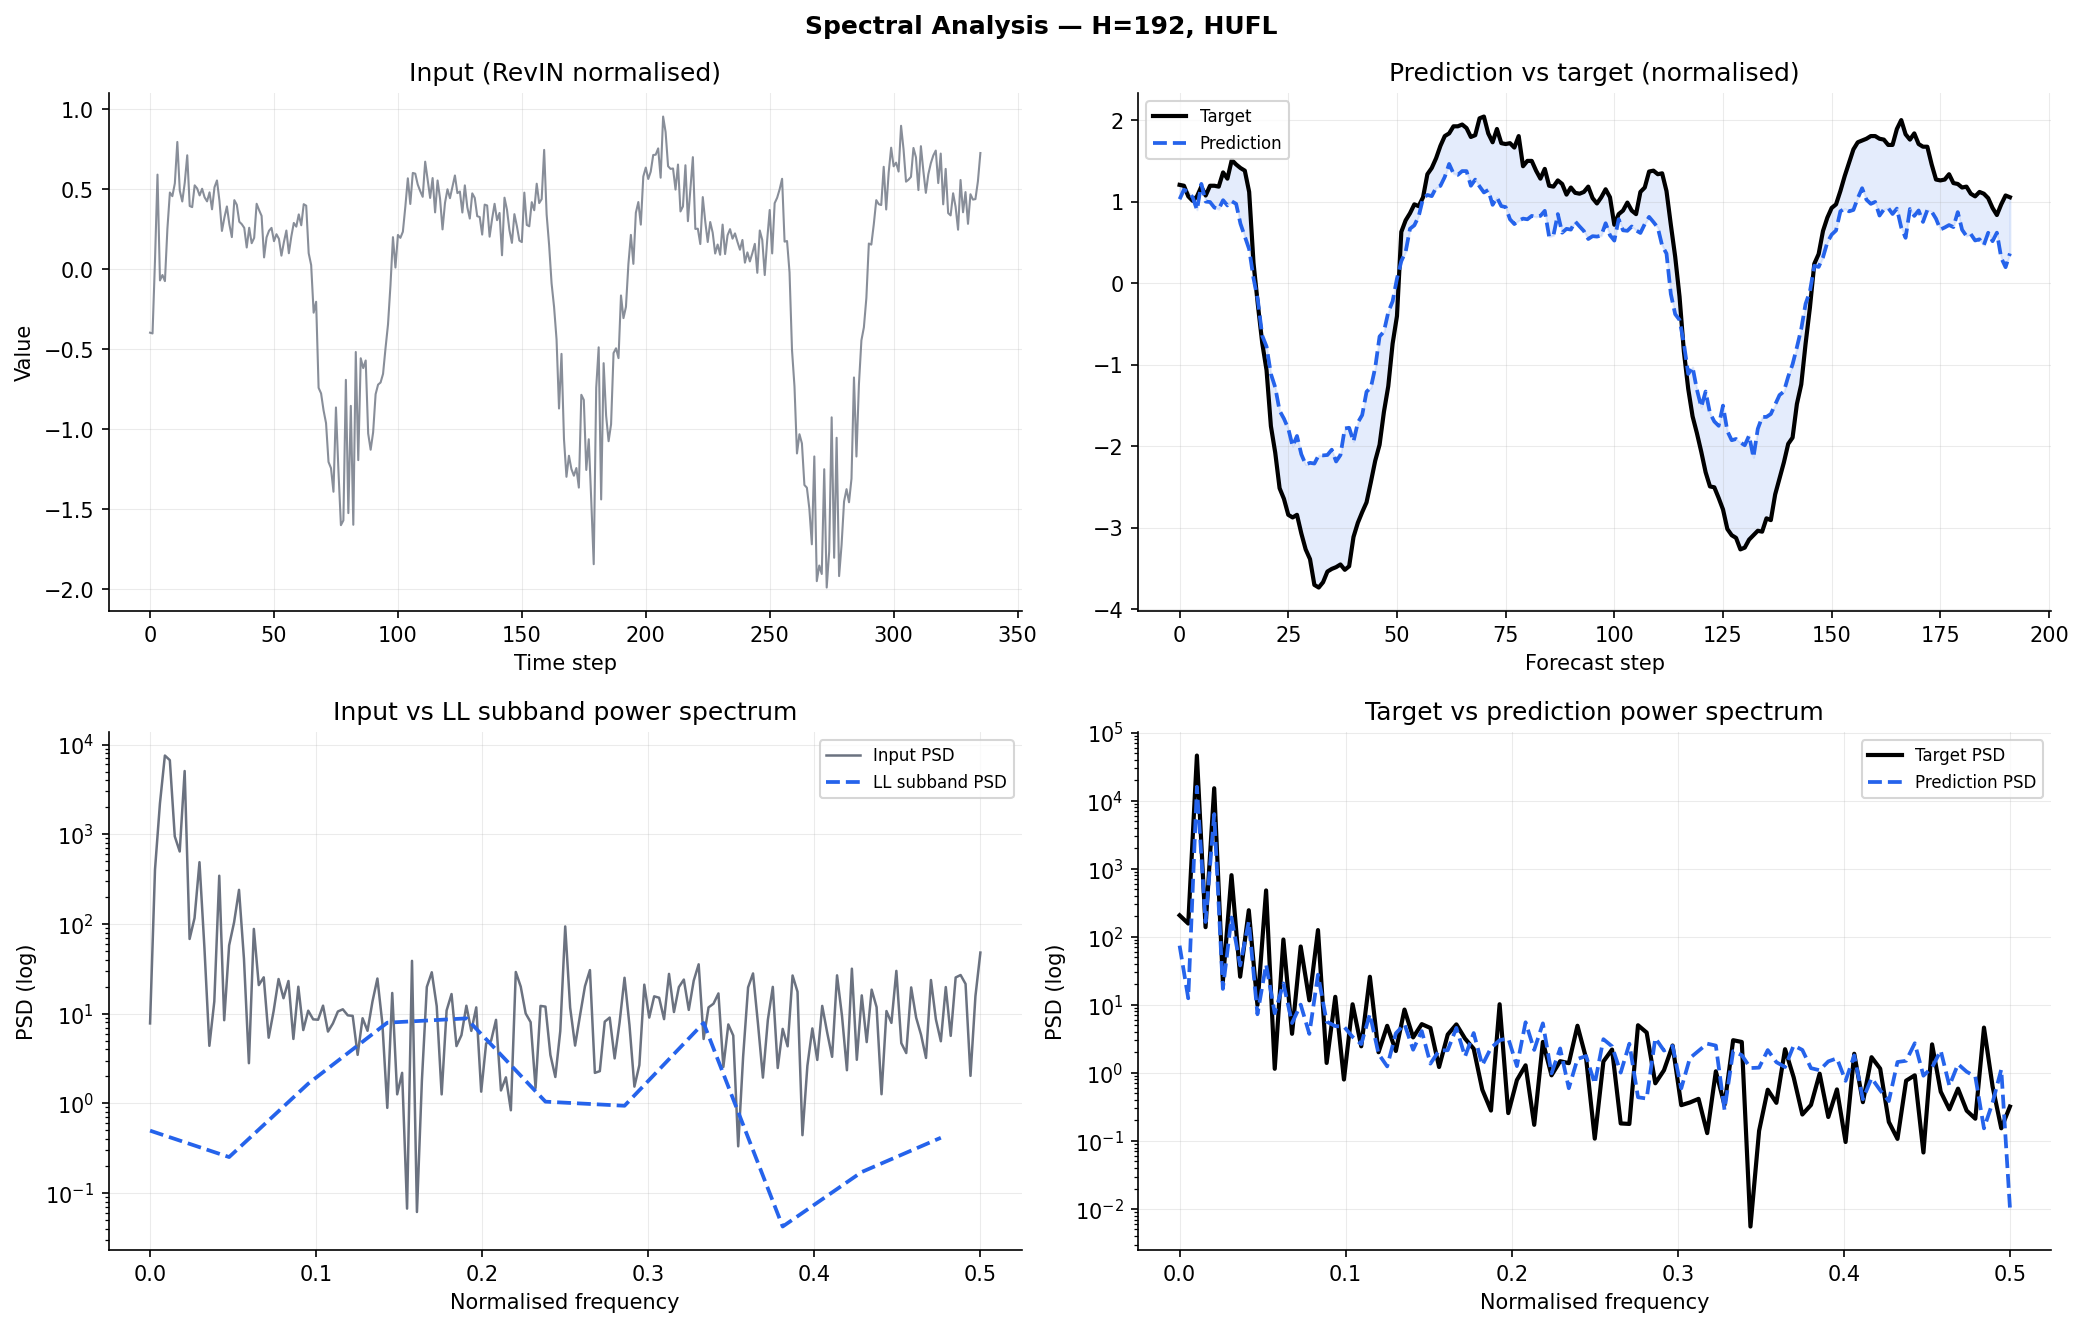
\includegraphics[width=\textwidth]{../report/plots-old/benchmarks/H192_spectral.png}
    \caption{$H=192$}
  \end{subfigure}
\end{figure}
\begin{figure}[H]
  \centering
  \begin{subfigure}[b]{0.48\textwidth}
    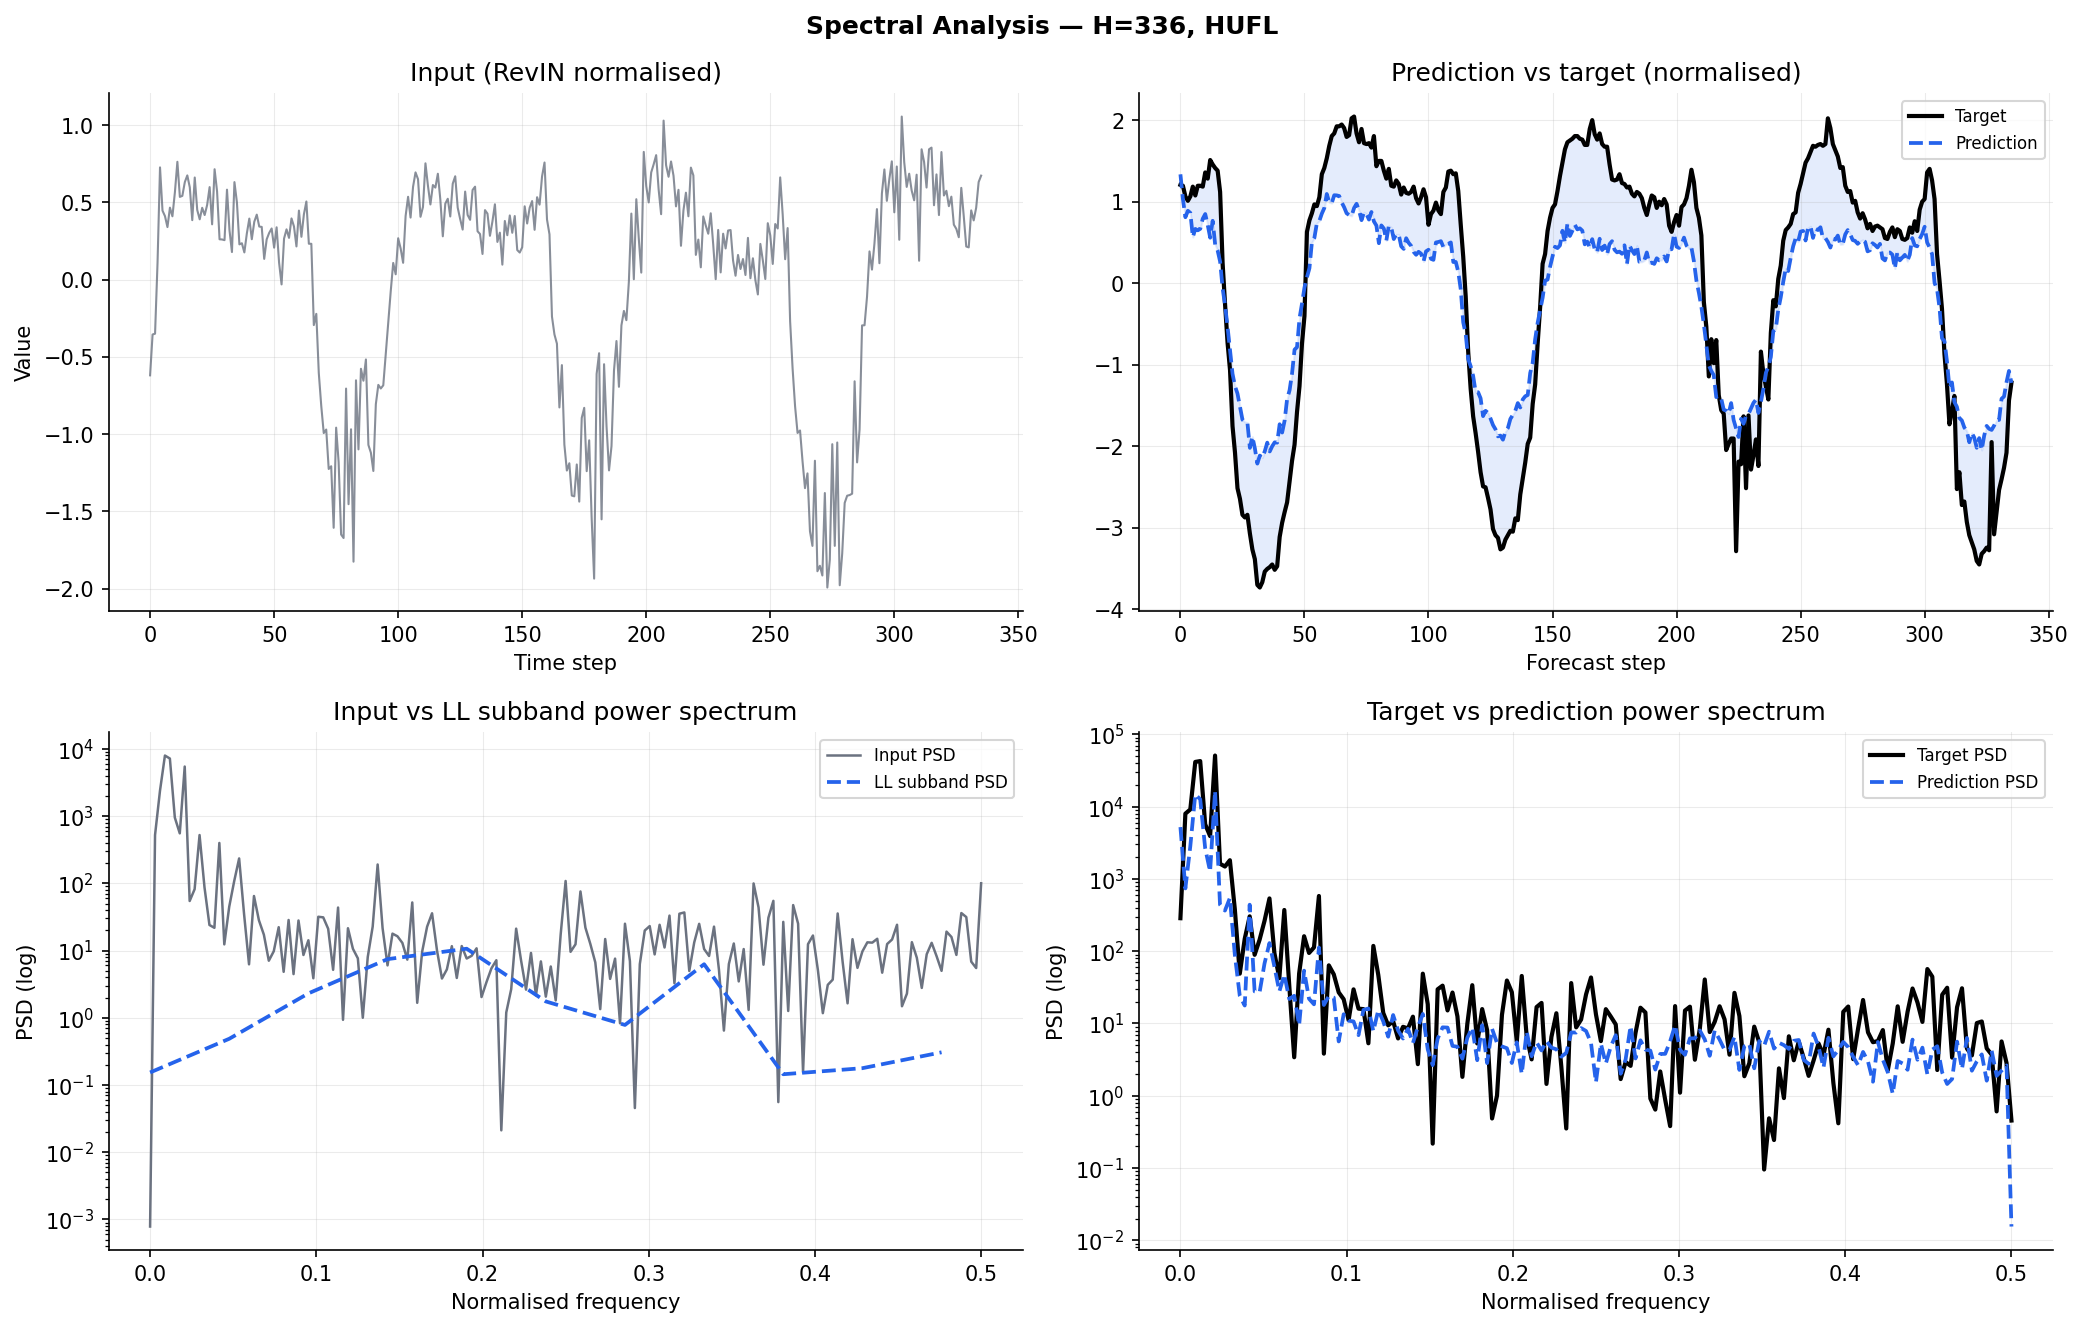
\includegraphics[width=\textwidth]{../report/plots-old/benchmarks/H336_spectral.png}
    \caption{$H=336$}
  \end{subfigure}\hfill
  \begin{subfigure}[b]{0.48\textwidth}
    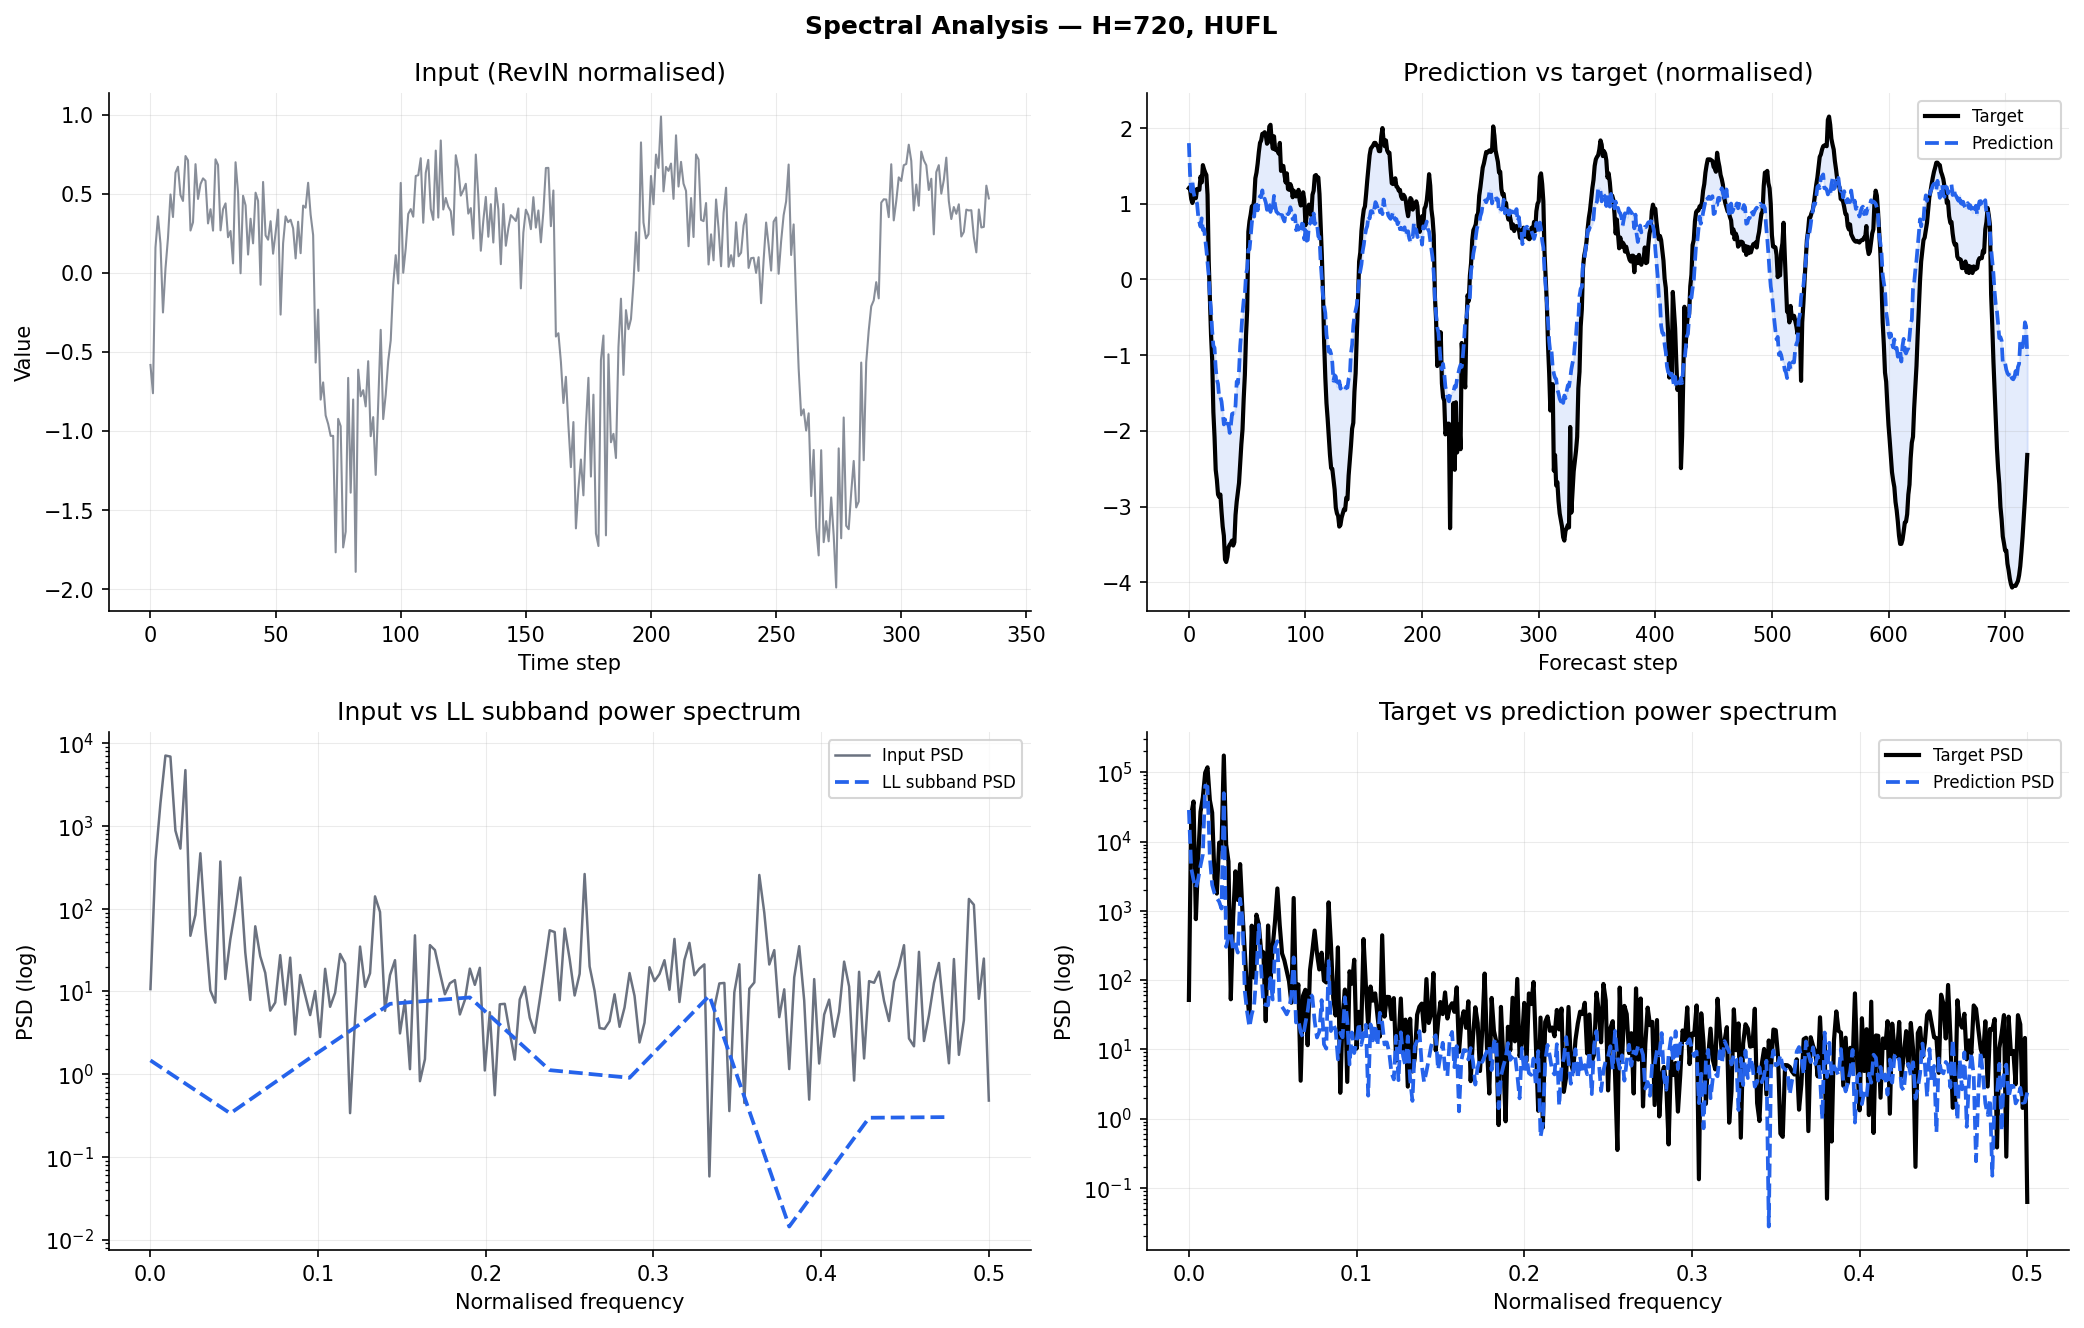
\includegraphics[width=\textwidth]{../report/plots-old/benchmarks/H720_spectral.png}
    \caption{$H=720$}
  \end{subfigure}
  \caption{Power spectral density of predictions vs.\ targets. The spectral penalty visibly aligns the prediction PSD with the target across all horizons.}
\end{figure}
\clearpage

\subsection*{C.3 Learned DWT Filter Dynamics}
\begin{figure}[H]
  \centering
  \begin{subfigure}[b]{0.48\textwidth}
    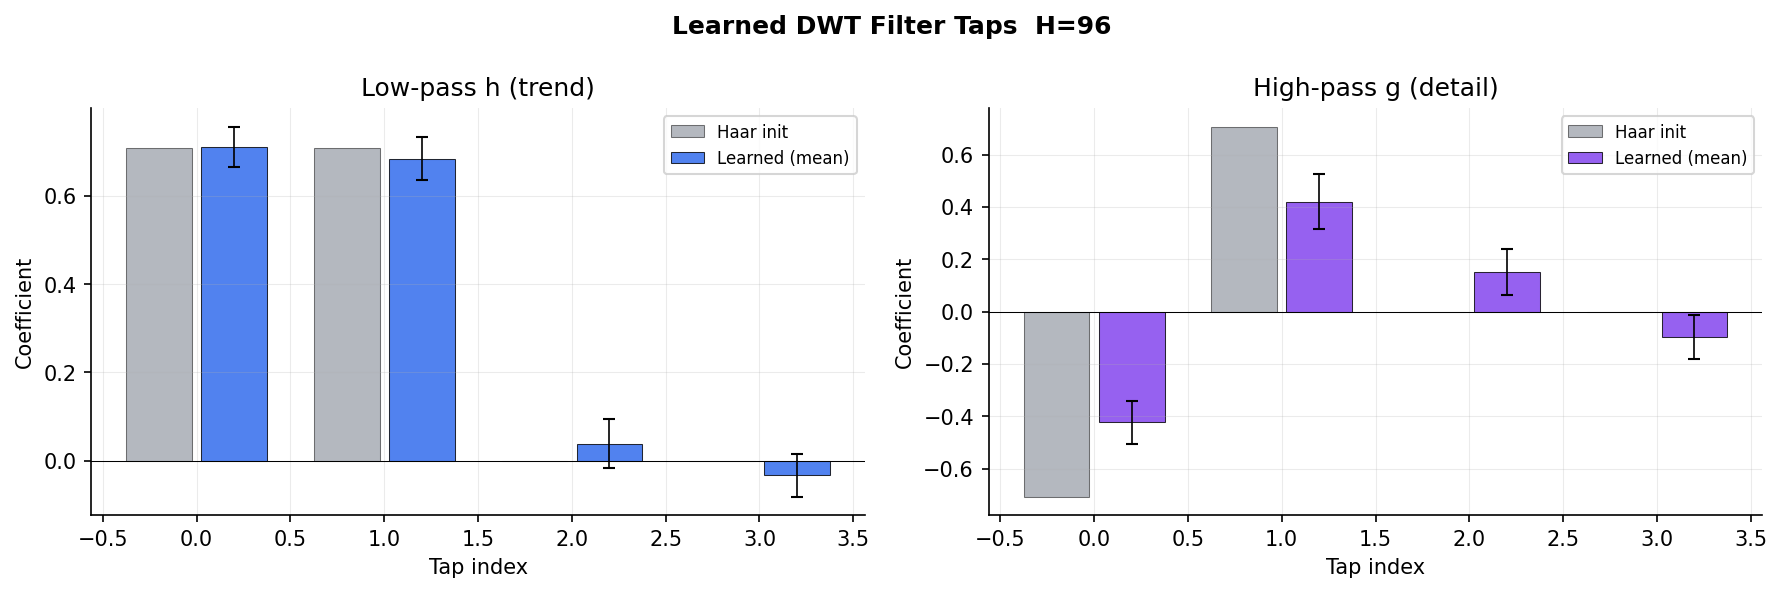
\includegraphics[width=\textwidth]{../report/plots-old/filters/H96_dwt_filters.png}
    \caption{Filter taps, $H=96$}
  \end{subfigure}\hfill
  \begin{subfigure}[b]{0.48\textwidth}
    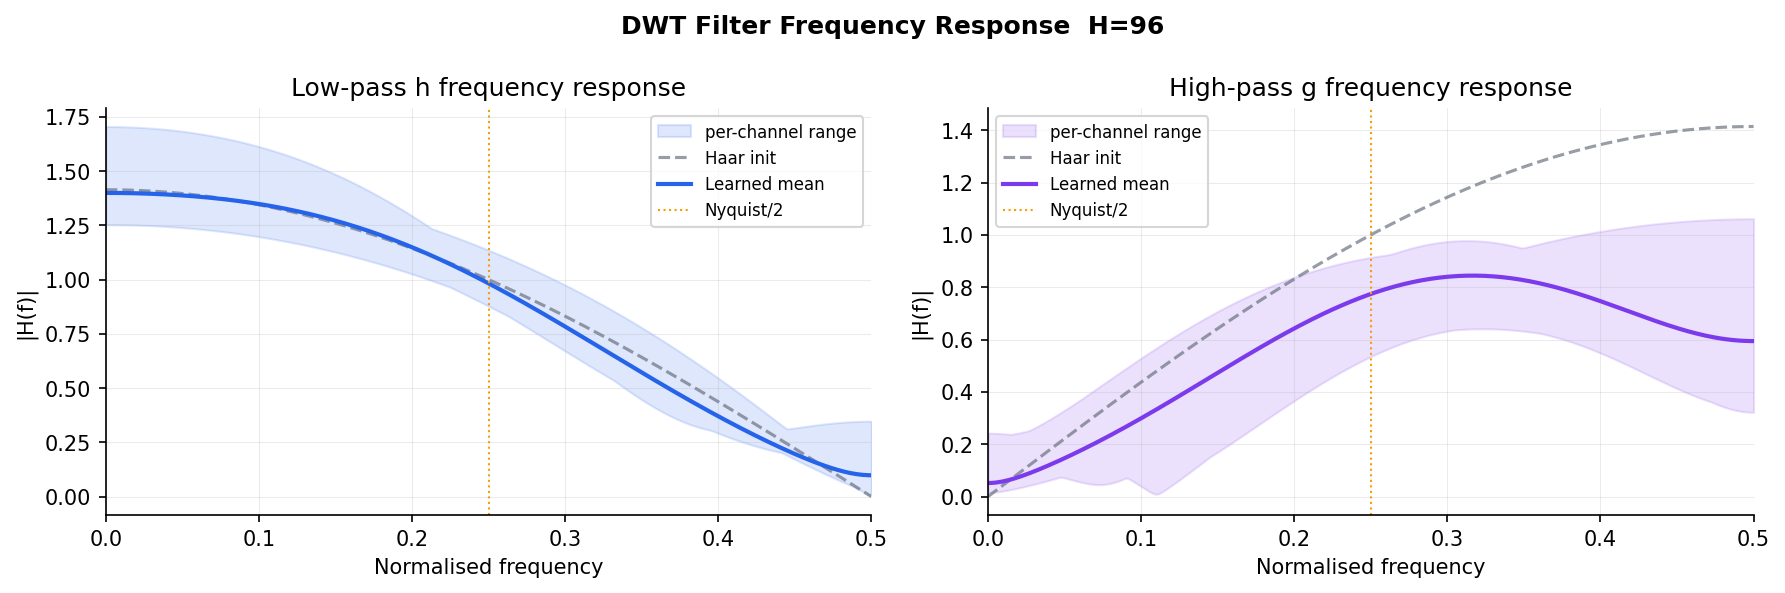
\includegraphics[width=\textwidth]{../report/plots-old/filters/H96_filter_spectrum.png}
    \caption{Frequency response, $H=96$}
  \end{subfigure}
\end{figure}
\begin{figure}[H]
  \centering
  \begin{subfigure}[b]{0.48\textwidth}
    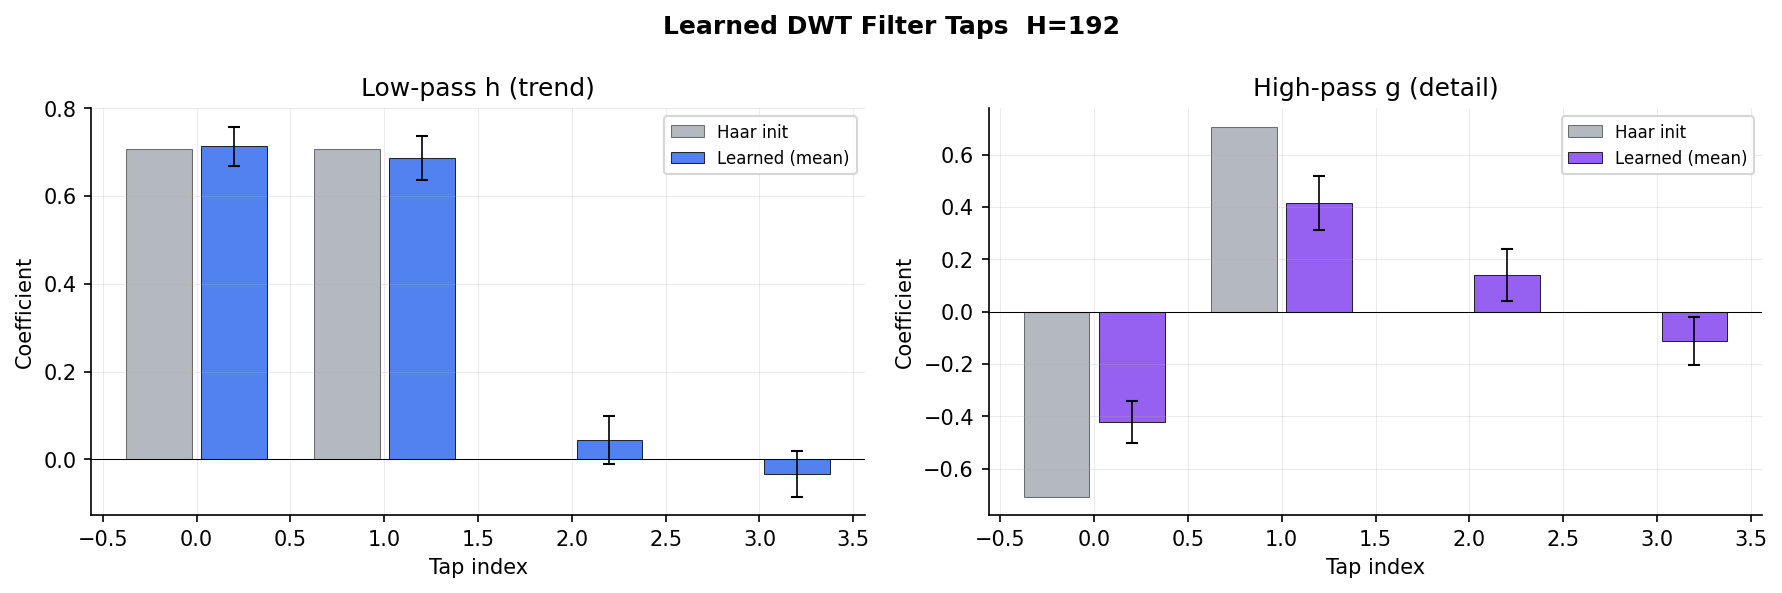
\includegraphics[width=\textwidth]{../report/plots-old/filters/H192_dwt_filters.png}
    \caption{Filter taps, $H=192$}
  \end{subfigure}\hfill
  \begin{subfigure}[b]{0.48\textwidth}
    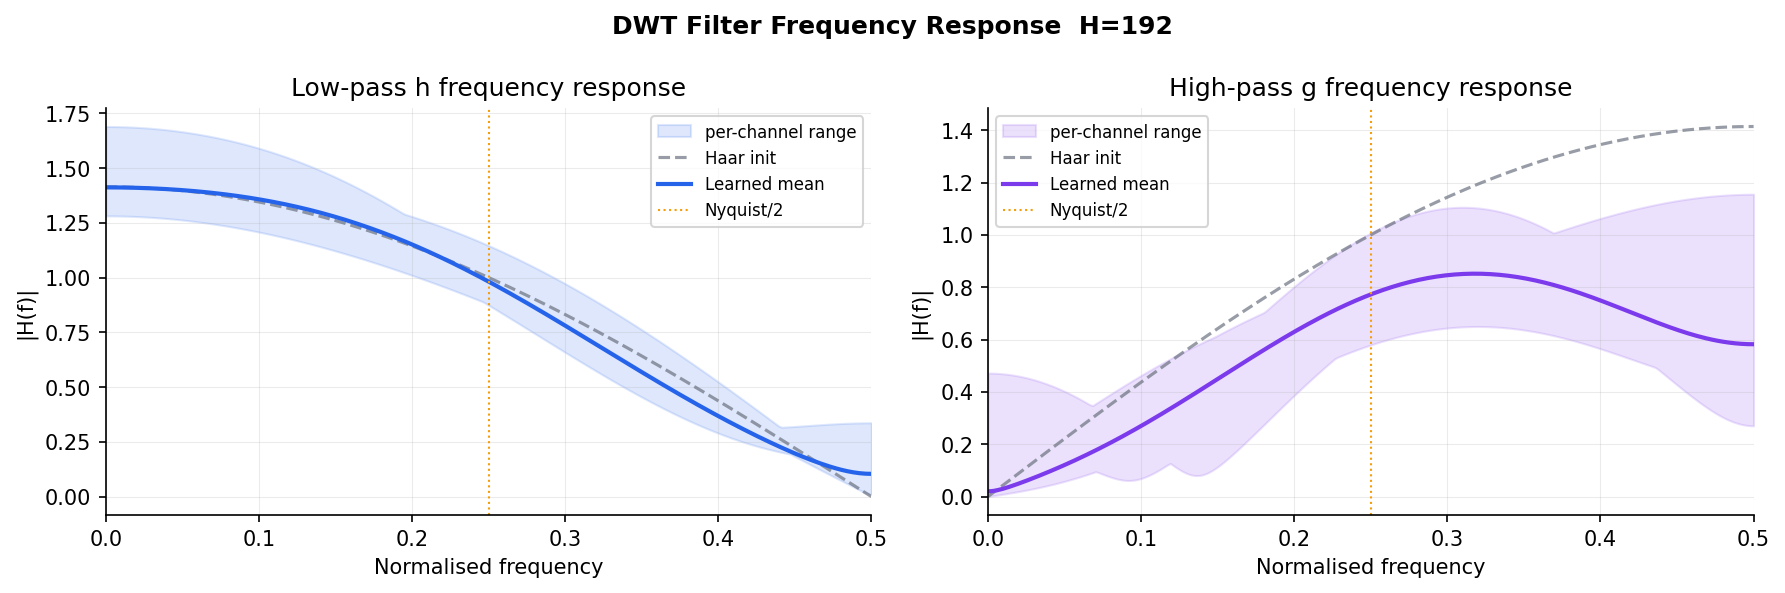
\includegraphics[width=\textwidth]{../report/plots-old/filters/H192_filter_spectrum.png}
    \caption{Frequency response, $H=192$}
  \end{subfigure}
\end{figure}
\begin{figure}[H]
  \centering
  \begin{subfigure}[b]{0.48\textwidth}
    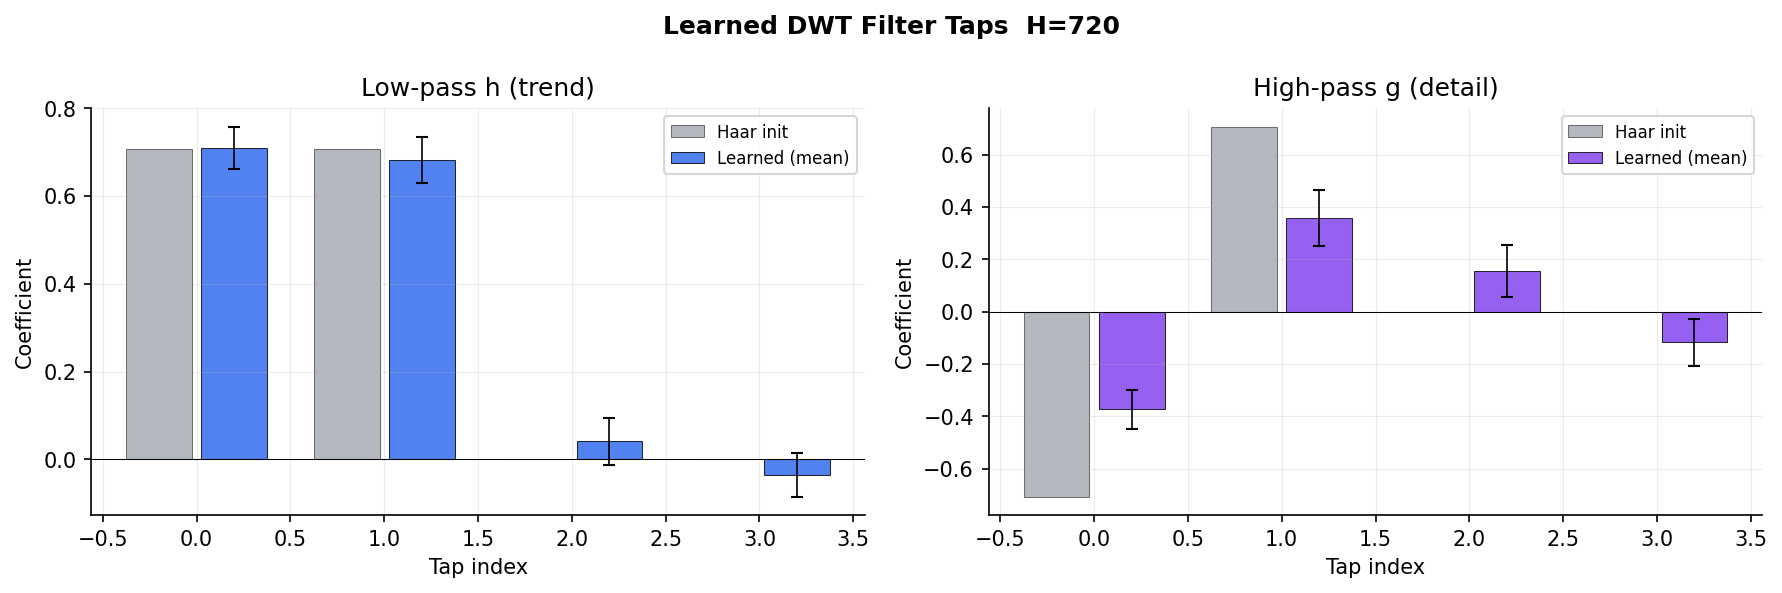
\includegraphics[width=\textwidth]{../report/plots-old/filters/H720_dwt_filters.png}
    \caption{Filter taps, $H=720$}
  \end{subfigure}\hfill
  \begin{subfigure}[b]{0.48\textwidth}
    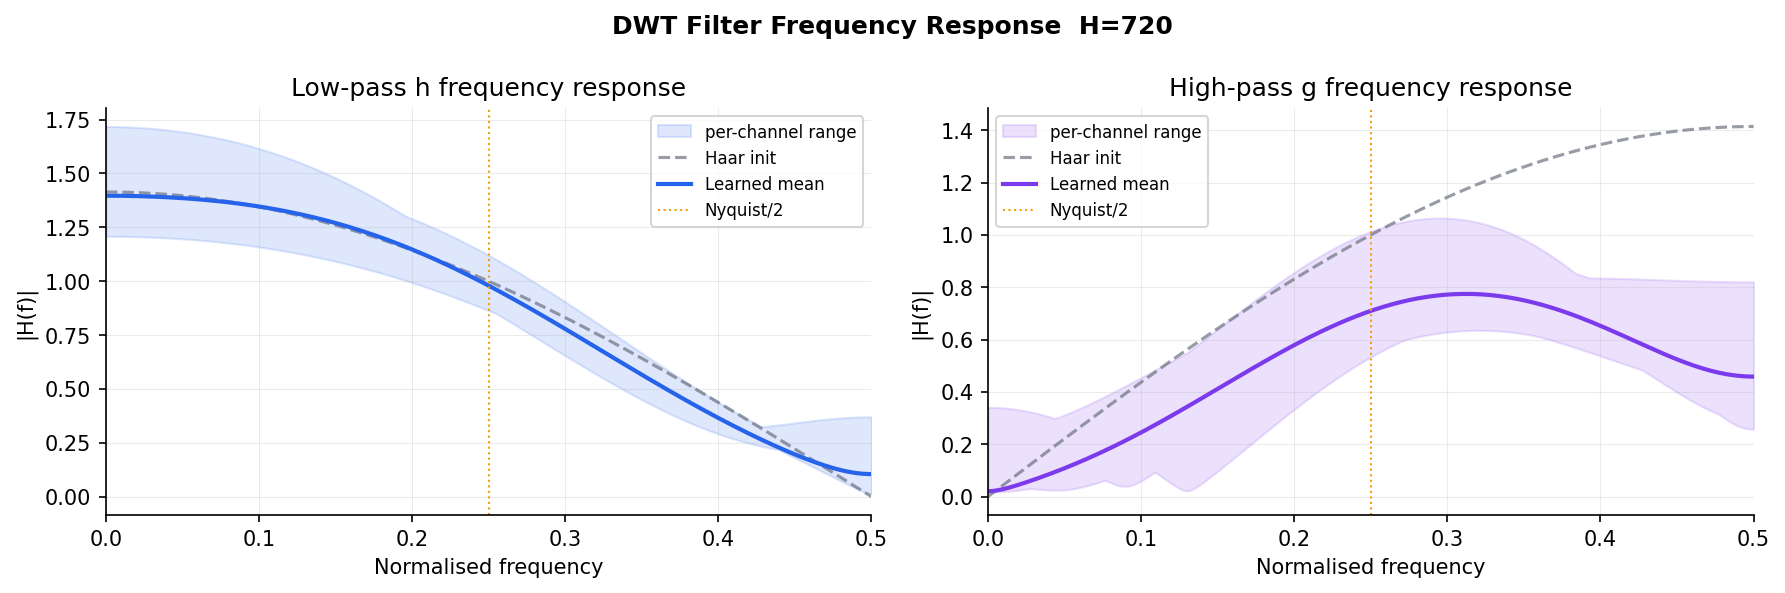
\includegraphics[width=\textwidth]{../report/plots-old/filters/H720_filter_spectrum.png}
    \caption{Frequency response, $H=720$}
  \end{subfigure}
  \caption{Learned filters deviate measurably from the Haar initialisation, confirming the wavelet module is actively learning. Per-channel norms remain consistent across horizons, suggesting filter adaptation is largely horizon-agnostic.}
\end{figure}
\clearpage

\subsection*{C.4 Learning Curves}
\begin{figure}[H]
  \centering
  \begin{subfigure}[b]{0.48\textwidth}
    
\includegraphics[width=\textwidth]{../report/plots-old/learning_curves/H96_curves.png}
    \caption{$H=96$}
  \end{subfigure}\hfill
  \begin{subfigure}[b]{0.48\textwidth}
    
\includegraphics[width=\textwidth]{../report/plots-old/learning_curves/H192_curves.png}
    \caption{$H=192$}
  \end{subfigure}
\end{figure}
\begin{figure}[H]
  \centering
  \begin{subfigure}[b]{0.48\textwidth}
    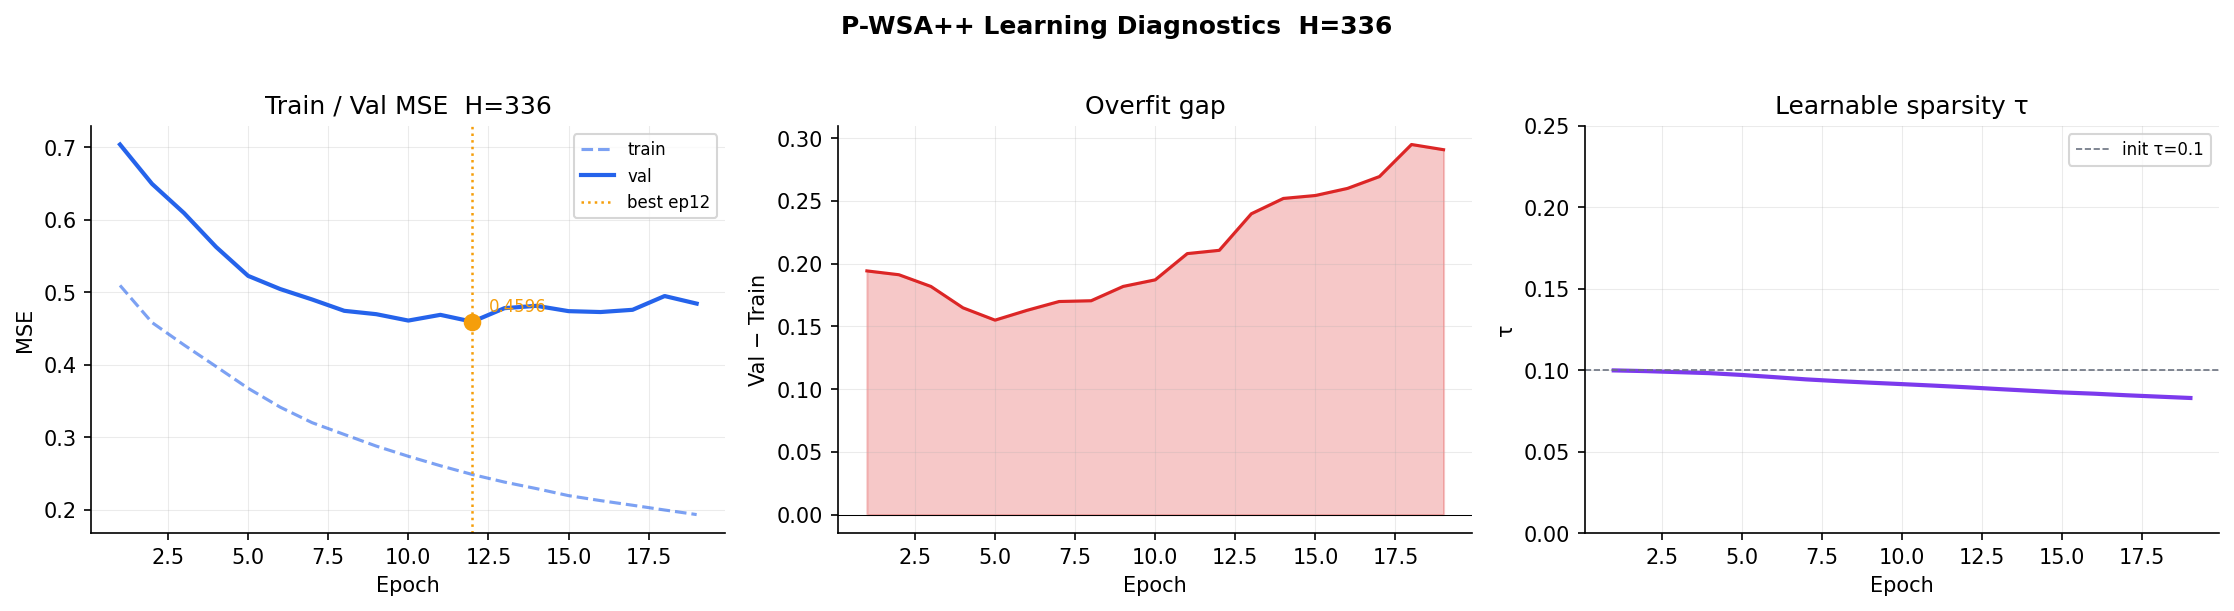
\includegraphics[width=\textwidth]{../report/plots-old/learning_curves/H336_curves.png}
    \caption{$H=336$}
  \end{subfigure}\hfill
  \begin{subfigure}[b]{0.48\textwidth}
    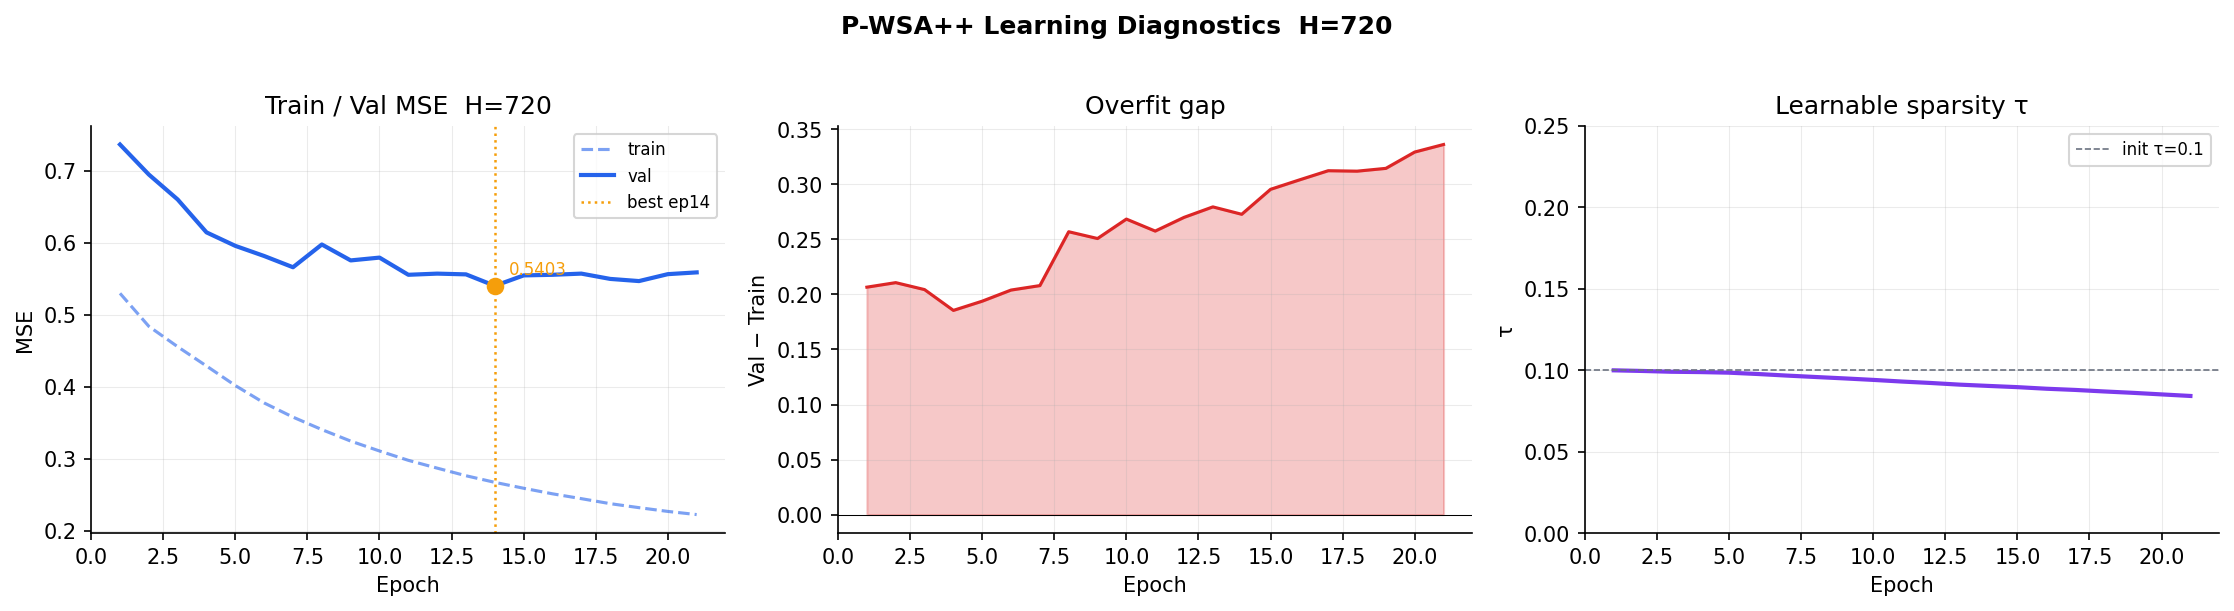
\includegraphics[width=\textwidth]{../report/plots-old/learning_curves/H720_curves.png}
    \caption{$H=720$}
  \end{subfigure}
  \caption{Training (dashed) and validation (solid) MSE. The warm-up phase is visible at the start; all horizons converge cleanly with minimal overfitting. The gap between horizons widens after epoch 20, consistent with accelerated information decay at long prediction windows.}
\end{figure}
\clearpage

\subsection*{C.5 Cross-Variate Analysis}
\begin{figure}[H]
  \centering
  \begin{subfigure}[b]{0.48\textwidth}
    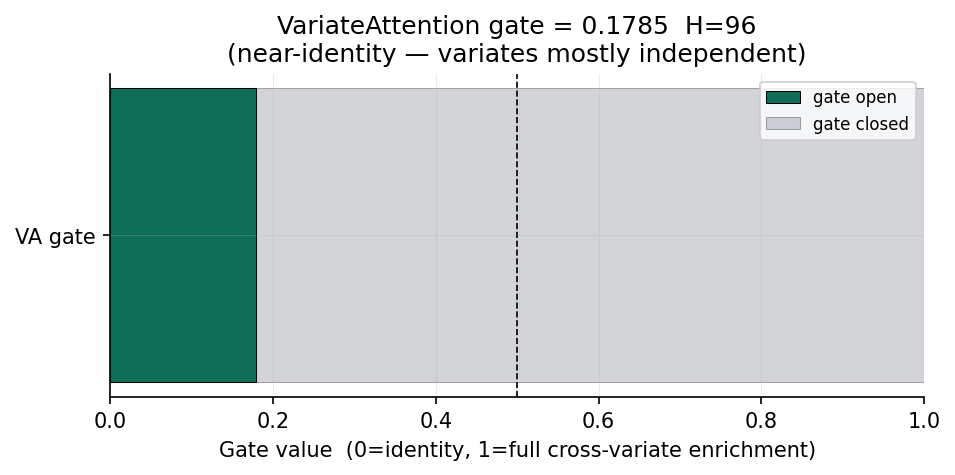
\includegraphics[width=\textwidth]{../report/plots-old/variate_graph/H96_variate_attn.png}
    \caption{Cross-variate attention, $H=96$}
  \end{subfigure}\hfill
  \begin{subfigure}[b]{0.48\textwidth}
    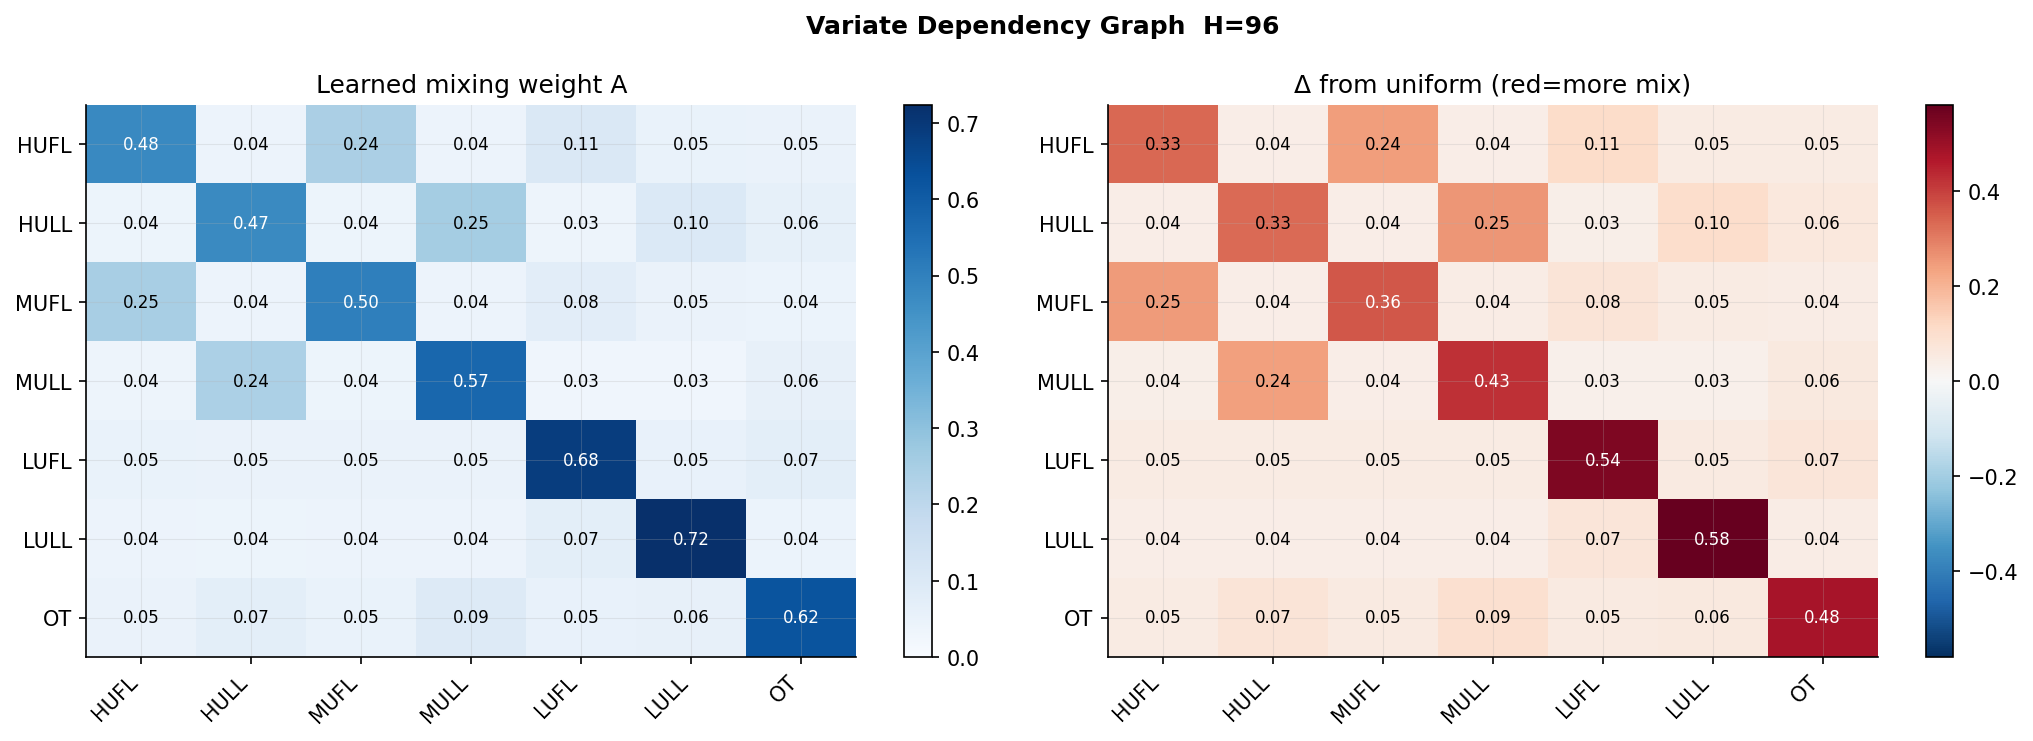
\includegraphics[width=\textwidth]{../report/plots-old/variate_graph/H96_adjacency.png}
    \caption{Adjacency matrix, $H=96$}
  \end{subfigure}
\end{figure}
\begin{figure}[H]
  \centering
  \begin{subfigure}[b]{0.48\textwidth}
    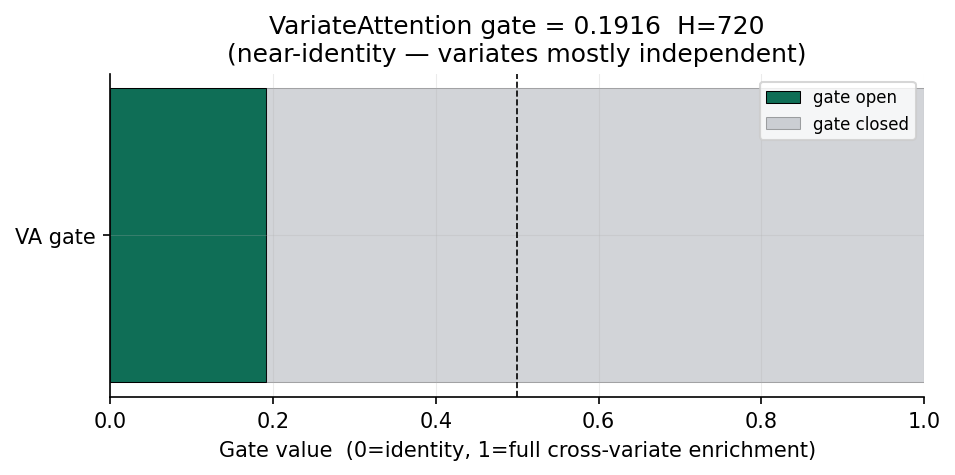
\includegraphics[width=\textwidth]{../report/plots-old/variate_graph/H720_variate_attn.png}
    \caption{Cross-variate attention, $H=720$}
  \end{subfigure}\hfill
  \begin{subfigure}[b]{0.48\textwidth}
    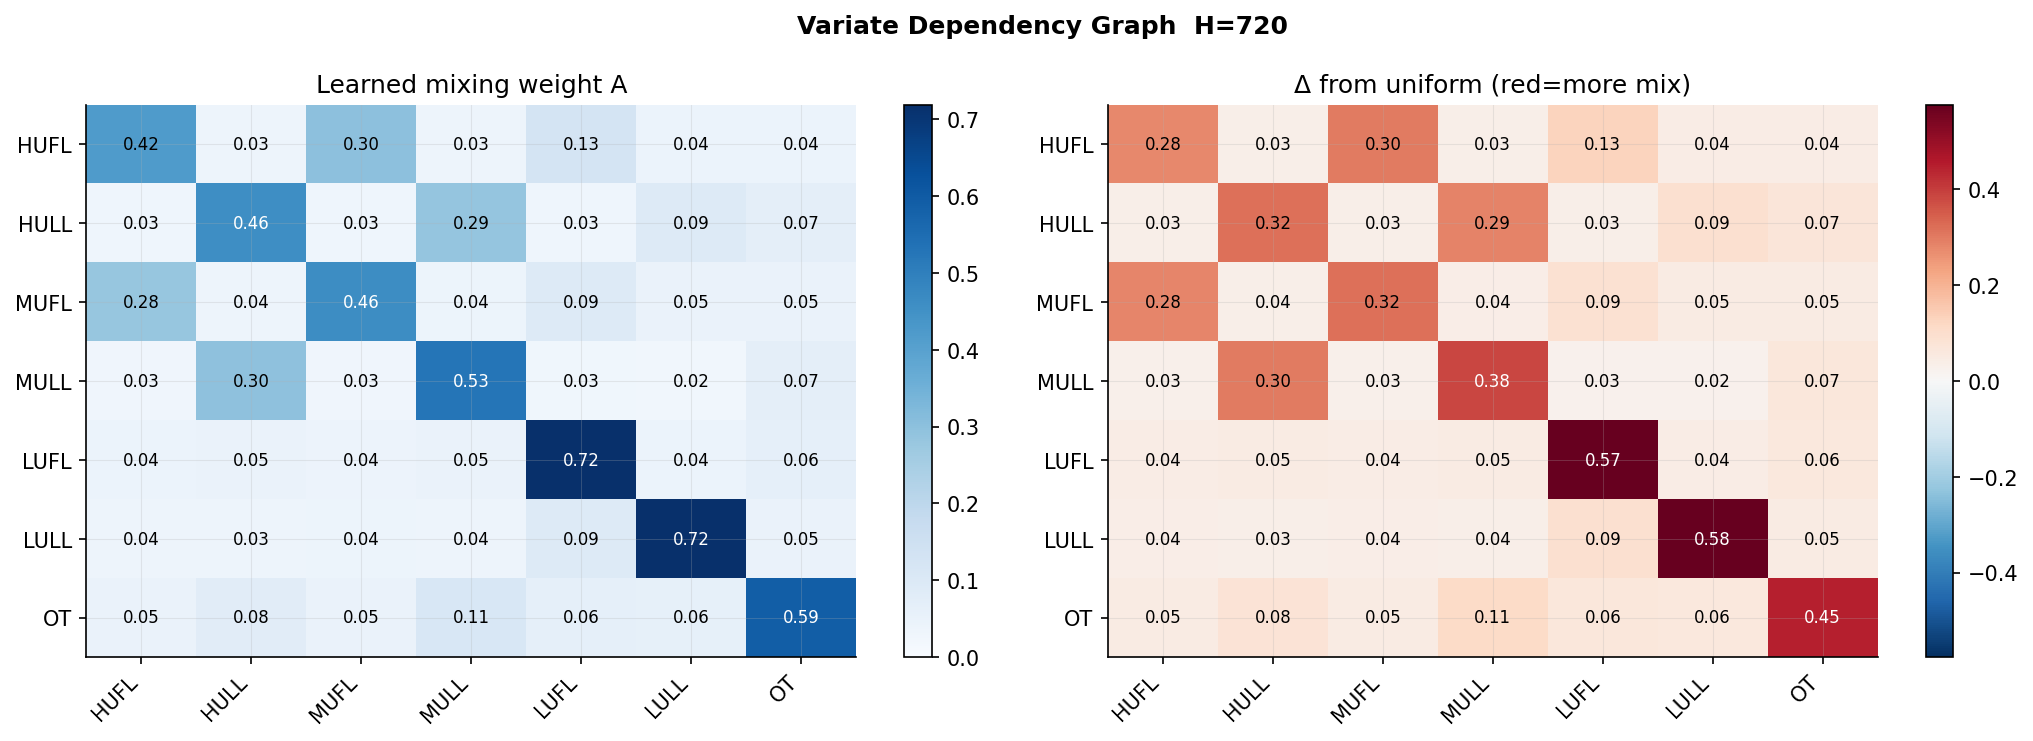
\includegraphics[width=\textwidth]{../report/plots-old/variate_graph/H720_adjacency.png}
    \caption{Adjacency matrix, $H=720$}
  \end{subfigure}
\end{figure}
\begin{figure}[H]
  \centering
  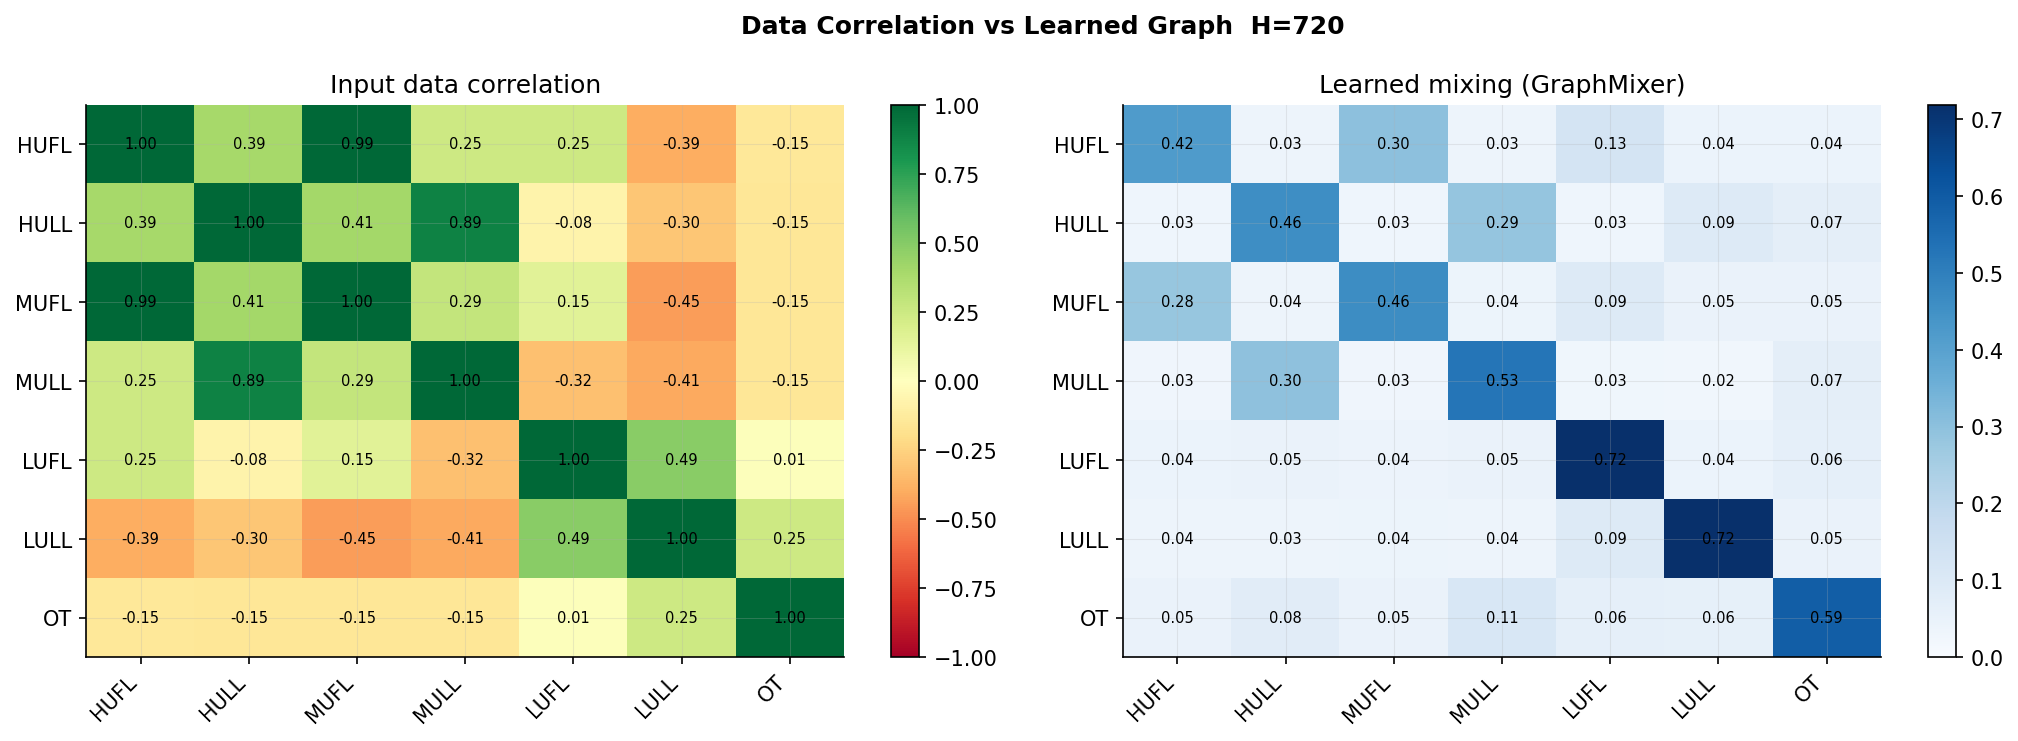
\includegraphics[width=0.7\textwidth]{../report/plots-old/variate_graph/correlation_vs_learned.png}
  \caption{Pearson correlation vs.\ learned variate interaction weights. The high agreement confirms that the Channel-Independence scheme implicitly captures cross-variate structure through the shared training loss.}
\end{figure}

\end{document}